%%%%%%%%%%%%%%%%%%%%%%%%%%%%%%%%%%%%%%%%%%%%%%%%%%%%%%%%%%%%
%%% LaPreprint: PREPRINT TEMPLATE
%%%%%%%%%%%%%%%%%%%%%%%%%%%%%%%%%%%%%%%%%%%%%%%%%%%%%%%%%%%%

% Here I could talk about what one should do in this document.
% Instead I'll refer you to the explore on your own and check the Github Repo. :-)
% Line spacing is 1.2 by default (can't be smaller).

%%%%%%%%%%%%%%%%%%%%%%%%%%%%%%%%%%%%%%%%%%%%%%%%%%%%%%%%%%%%
%%% PREAMBLE
%%%%%%%%%%%%%%%%%%%%%%%%%%%%%%%%%%%%%%%%%%%%%%%%%%%%%%%%%%%%

% Declare document class
\documentclass[9pt,biorxiv,doublespacing,lineno]{lapreprint}
% Choose between "biorxiv", "medrxiv", "arxiv" and "chemrxiv". Otherwise defaults "Preprint".
% Choose between "blue" and "red" colour scheme. Defaults to "blue".
% Use the "onehalfspacing" option for 1.5 line spacing.
% Use the "doublespacing" option for 2.0 line spacing.
% Use the "lineno" option for line numbers.
% Use the "endfloat" option to place floats after the bibliography.

% Import packages
% \usepackage{lipsum}     % Required to insert dummy text
\usepackage[version=4]{mhchem} % For chemical notation
\usepackage{siunitx}    % For SI units
\usepackage{pdflscape}  % For putting pages in landscape mode
\usepackage{rotating}   % For rotating specific elements
\usepackage{textgreek}  % Greek symbols
\usepackage{gensymb}    % Symbols
\usepackage[misc]{ifsym} % For the \Letter symbol
\usepackage{orcidlink}  % For the \orcidlink
\usepackage{listings}   % For inserting code chunks
\usepackage{colortbl}   % For Knitr table colouring
\usepackage{tabularx}   % For making Knitr tables compatible
\usepackage{longtable}  % For multi-page tables
\usepackage{multirow}
\usepackage{snotez}     % For sidenote environments. enotez for endnotes
\usepackage{csquotes}   % For language-based quote rules (helps BiBLaTeX)

% Custom packages
\usepackage{threeparttable}

\providecommand{\tightlist}{% Command for list
\setlength{\itemsep}{0pt}\setlength{\parskip}{0pt}}

%% Make sure that the picture stay on the page
\makeatletter
\def\maxwidth{\ifdim\Gin@nat@width>\linewidth\linewidth\else\Gin@nat@width\fi}
\def\maxheight{\ifdim\Gin@nat@height>\textheight\textheight\else\Gin@nat@height\fi}
\makeatother
% Scale images if necessary, so that they will not overflow the page
% margins by default, and it is still possible to overwrite the defaults
% using explicit options in \includegraphics[width, height, ...]{}
\setkeys{Gin}{width=\maxwidth,height=\maxheight,keepaspectratio}

\makeatletter
\@ifpackageloaded{subfig}{}{\usepackage{subfig}}
\@ifpackageloaded{caption}{}{\usepackage{caption}}
\captionsetup[subfloat]{margin=0.5em}
\AtBeginDocument{%
\renewcommand*\figurename{Figure}
\renewcommand*\tablename{Table}
}
\AtBeginDocument{%
\renewcommand*\listfigurename{List of Figures}
\renewcommand*\listtablename{List of Tables}
}
\newcounter{pandoccrossref@subfigures@footnote@counter}
\newenvironment{pandoccrossrefsubfigures}{%
\setcounter{pandoccrossref@subfigures@footnote@counter}{0}
\begin{figure}\centering%
\gdef\global@pandoccrossref@subfigures@footnotes{}%
\DeclareRobustCommand{\footnote}[1]{\footnotemark%
\stepcounter{pandoccrossref@subfigures@footnote@counter}%
\ifx\global@pandoccrossref@subfigures@footnotes\empty%
\gdef\global@pandoccrossref@subfigures@footnotes{{##1}}%
\else%
\g@addto@macro\global@pandoccrossref@subfigures@footnotes{, {##1}}%
\fi}}%
{\end{figure}%
\addtocounter{footnote}{-\value{pandoccrossref@subfigures@footnote@counter}}
\@for\f:=\global@pandoccrossref@subfigures@footnotes\do{\stepcounter{footnote}\footnotetext{\f}}%
\gdef\global@pandoccrossref@subfigures@footnotes{}}
\@ifpackageloaded{float}{}{\usepackage{float}}
\floatstyle{ruled}
\@ifundefined{c@chapter}{\newfloat{codelisting}{h}{lop}}{\newfloat{codelisting}{h}{lop}[chapter]}
\floatname{codelisting}{Listing}
\newcommand*\listoflistings{\listof{codelisting}{List of Listings}}
\makeatother

%% pandoc-tablenos: required package
\usepackage{caption}

%% pandoc-tablenos: environment to disable table caption prefixes
\makeatletter
\newcounter{tableno}
\newenvironment{tablenos:no-prefix-table-caption}{
  \caption@ifcompatibility{}{
    \let\oldthetable\thetable
    \let\oldtheHtable\theHtable
    \renewcommand{\thetable}{tableno:\thetableno}
    \renewcommand{\theHtable}{tableno:\thetableno}
    \stepcounter{tableno}
    \captionsetup{labelformat=empty}
  }
}{
  \caption@ifcompatibility{}{
    \captionsetup{labelformat=default}
    \let\thetable\oldthetable
    \let\theHtable\oldtheHtable
    \addtocounter{table}{-1}
  }
}
\makeatother

% Make declarations
\DeclareSIUnit\Molar{M}

% Please note that these options may affect formatting. 

%%%%%%%%%%%%%%%%%%%%%%%%%%%%%%%%%%%%%%%%%%%%%%%%%%%%%%%%%%%%
%%% BIBLIOGRAPHY
%%%%%%%%%%%%%%%%%%%%%%%%%%%%%%%%%%%%%%%%%%%%%%%%%%%%%%%%%%%%
\usepackage[			% use biblatex for bibliography
	backend=biber,      % use biber or bibtex backend
  style=authoryear,   % choose style
	hyperref=true,	    % activate hyperref support
	alldates=year,      % only show year (not month)
]{biblatex}

% Update to your bibliography file
\addbibresource{bibliography.bib}

%%%%%%%%%%%%%%%%%%%%%%%%%%%%%%%%%%%%%%%%%%%%%%%%%%%%%%%%%%%%
%%% ARTICLE SETUP
%%%%%%%%%%%%%%%%%%%%%%%%%%%%%%%%%%%%%%%%%%%%%%%%%%%%%%%%%%%%

% Paper title
\title{Essential ingredients in Joint Species Distribution Models:
influence on interpretability, explanatory and predictive power}

% Authors - you can use \orcidlink{} and \authfn{} - see contribution note

% You need to have white spaces around the \orcidlink{} command
% otherwise, LaTeX will raise errors
\author[ \orcidlink{0000-0001-6217-5891} 1\Letter]{Clément Violet}
\author[ \orcidlink{0000-0002-5692-7660} 1]{Aurélien Boyé}
\author[ \orcidlink{0000-0002-1170-5343} 1]{Mathieu Chevalier}
\author[ \orcidlink{0000-0002-4158-7560} 2]{Olivier Gauthier}
\author[ \orcidlink{0000-0002-3107-6740} 3]{Jacques Grall}
\author[ \orcidlink{0000-0002-8152-4273} 1]{Martin P. Marzloff}

% Affiliations
\affil[1]{IFREMER, Centre de Bretagne, DYNECO LEBCO, Plouzané, France}
\affil[2]{Laboratoire des Sciences de l'Environnement Marin (LEMAR) UMR
6539 CNRS UBO IRD IFREMER, Institut Universitaire Européen de la Mer,
Université de Bretagne Occidentale, Plouzané, France}
\affil[3]{Observatoire des Sciences de l'Univers, UMS 3113, Institut
Universitaire Européen de la Mer, Plouzané, France}

% Other metadata. Feel free to add your own
\metadata[]{\Letter\hspace{.5ex} For correspondence}{\href{mailto:}{clement.violet@ifremer.fr}}
\metadata[]{Present address}{IFREMER, Centre de Bretagne, DYNECO LEBCO,
Plouzané 29280, France.}
\metadata[]{Keywords}{Community assembly, Explanatory
power, Interpretability, Joint Species Distribution Model, jSDM, Model
Performances, Predictive power, Species Distribution Model}
\metadata[]{Data availability}{\href{https://github.com/clementviolet/mee-Essential-ingredients-JSDM}{Github: Clement Violet}}
\metadata[]{Competing interests}{The authors declare no competing
interests.}
\metadata[]{Funding}{This work benefits from funding from IFREMER.}
% \metadata[\authfn{1}\authfn{2}\authfn{3}]{}{Here's a few symbols to denote contribution specifics, e.g. authors who contributed equally to the work.}

% Surname of the lead author(s) for the running footer
\leadauthor{Violet}
\shorttitle{Essential ingredients in Joint Species Distribution Models}

%%%%%%%%%%%%%%%%%%%%%%%%%%%%%%%%%%%%%%%%%%%%%%%%%%%%%%%%%%%%
%%% ARTICLE START
%%%%%%%%%%%%%%%%%%%%%%%%%%%%%%%%%%%%%%%%%%%%%%%%%%%%%%%%%%%%

\begin{document}
\maketitle

\begin{abstract}

\begin{enumerate}
\def\labelenumi{\arabic{enumi}.}
\item
  \emph{Joint Species Distribution Models} (\emph{jSDM}) are
  increasingly used to explain and predict biodiversity patterns.
  \emph{jSDMs} account for species co-occurrence patterns and can
  include phylogeny or functional traits to better capture the processes
  shaping communities. Yet, several factors may alter the
  interpretability and predictive ability of \emph{jSDMs} : missing
  abiotic predictors, omitting ecologically-important species, or
  increasing the number of model parameters by adding phylogeny and/or
  trait information.
\item
  We developed a novel framework to comprehensively assess the
  interpretability, explanatory and predictive power of \emph{jSDMs} at
  both species and community levels. We compared performances of four
  alternative model formulations : (1) a \emph{Benchmark} \emph{jSDM}
  with only abiotic predictors and residual co-occurrence patterns, (2)
  a \emph{jSDM} adding phylogeny to the \emph{Benchmark}, (3) a
  \emph{jSDM} adding traits to model 2, and (4) the \emph{Benchmark}
  \emph{jSDM} with additional non-target species that are not of direct
  interest but potentially interact with the target assemblage. Models
  were fitted on both presence/absence and abundance data for 99 target
  polychaete species sampled in two coastal habitats over 500km and 8
  years, along with information on 179 non-target species and traits
  data for the target species.
\item
  For both presence/absence and abundance data, explanatory power was
  good for all models but their interpretability and predictive power
  varied. Relative to the \emph{Benchmark} model, predictive errors on
  species abundances decreased by 95\% or 53\%, when including
  non-target species, or phylogeny, respectively. These differences
  across models relate to changes in both species-environment
  relationships and residual co-occurrence patterns. While considering
  trait data did not improve explanatory or predictive power, it
  facilitated interpretation of trait-mediated species response to
  environmental gradients.
\item
  This study demonstrates that any \emph{jSDM} formulation comes with
  tradeoffs between either explaining or predicting the occurrence or
  abundance of species. Hence, it highlights the need to compare
  alternative model formulations using the original and comprehensive
  assessment framework proposed in this study. Overall, this work
  contributes to a better understanding of \emph{jSDM}s' performances
  across multiple facets and provides insights and tools for model
  selection based on specific objectives and available data.
\end{enumerate}
\end{abstract}

\hypertarget{introduction}{%
\section{Introduction}\label{introduction}}

Community ecology aims at describing, explaining, and predicting changes
in communities \autocite{Tredennick_2021}. Understanding the processes
that determine species distribution is a prerequisite to characterize
and predict community structure and associated ecological dynamics,
which is critical to inform effective management or restoration measures
in a rapidly changing world \autocites[ ]{Dietze_2018}{Brudvig_2022}.
\emph{Joint Species Distribution Models} (\emph{jSDM}) are particularly
well-suited tools to address these challenges, whether to characterize
the processes that shape observed communities \autocites[
]{Warton_2015}{Ovaskainen_2017b}, or to predict future changes in
species assemblages \autocites[ ]{Norberg_2019}{Pollock_2020}.

\emph{jSDMs} are multivariate (i.e.~multi-species) extensions of
\emph{Species Distribution Models} (\emph{SDMs}), which have been
broadly applied over the past decades - across all terrestrial and
marine realms - to understand and predict both species occurrences
\autocites[ ]{Elith_2006}{Norberg_2019} and species abundances
\autocites[ ]{Howard_2014}{Waldock_2022} using a set of covariates
(e.g.~climatic variables). Relative to \emph{SDMs}, \emph{jSDMs}
explanatory power can benefit from accounting for species assembly rules
\autocite{Ovaskainen_2017a}. In particular, relative to single-species
\emph{SDMs} that only consider the abiotic niche of species (i.e.~the
Grinellian niche), \emph{jSDM} can theoretically also account for
interspecific interactions (i.e.~the Eltonian niche).

In \emph{jSDMs}, the variability in community composition not explained
by covariates is captured by a residual covariance matrix representing
species co-occurrence patterns potentially representing biotic
interactions \autocite{Ovaskainen_2017a}. This feature is highly
attractive to ecologists because it provides a way to disentangle the
relative influence of abiotic and biotic processes on biodiversity
patterns \autocite{Godsoe_2017} while also improving model's predictive
power \autocites[ ]{Giannini_2013}{Staniczenko_2017}. However, in
practice, inferring and interpreting residual co-occurrence patterns
using \emph{jSDMs} remains challenging for several reasons \autocites[
]{Blanchet_2020}{Holt_2020}.

First, while \emph{jSDMs} have been applied to a large number of species
presence/absence datasets \autocites[ ]{Norberg_2019}[
]{Wilkinson_2019}{Wilkinson_2020}, simulation studies showed that
inferred co-occurrence networks do not necessarily provide evidence for
species interactions \autocites[ ]{Dormann_2018}{Blanchet_2020} but only
capture spatial and temporal associations between species
\autocite{Keil_2021}. Some authors speculated that \emph{jSDMs} applied
to abundance data - instead of presence/absence data - could provide a
better proxy for biotic interactions \autocites[
]{Blanchet_2020}{Momal_2020}. Accordingly, \emph{jSDM} have increasingly
been applied to abundance data \autocites[ ]{Hui_2016}[
]{Ovaskainen_2017a}{Chiquet_2021}. While challenges related to modelling
abundance data was recently explored in the context of species
distribution modelling \autocite{Waldock_2022}, the predictive and the
explanatory power of \emph{jSDM} fitted to abundance data remains
relatively untested compared to presence/absence data \autocites[
]{Norberg_2019}{Wilkinson_2020}.

Second, regardless of the type of data considered (i.e.~presence/absence
or abundance), several factors may limit or affect the interpretability
and predictive ability of \emph{jSDM}. For instance, co-occurrence
patterns estimated in \emph{jSDM} are affected by unaccounted
environmental variables implying that \emph{jSDMs} cannot fully separate
the environmental and the biotic niche of species \autocites[
]{Blanchet_2020}{Poggiato_2021}. Beyond missing environmental
predictors, accounting for extra species that can influence the target
community (e.g.~competitors) is key to improve \emph{jSDMs}' inference
and predictions. However, because many ecological studies only focus on
particular taxonomic groups \autocites[ ]{Pollock_2014}{Hakkila_2018}
and disregard non-target taxa, co-occurrence patterns estimated from
\emph{jSDMs} are almost always skewed by missing ecological actors
\autocite{Momal_2021}. How this bias affects the predictive ability of
jSDM remains untested.

Finally, similar to \emph{SDMs}, \emph{jSDMs} can theoretically be
extended to include additional sources of information about modelled
species \autocites[ ]{Niku_2019}{Ovaskainen_2017a}. For instance,
accounting for phylogenetic relationships between species
\autocite{Ives_2011} or for the link between functional traits and
environmental responses \autocite{Pollock_2012} can improve both the
explanatory and the predictive powers of \emph{SDMs} \autocites[
]{Morales-Castilla_2017}{Vesk_2021}. These findings support the
hypothesis that similar species, in terms of traits and/or recent
evolutionary history, usually share similar environmental preferences.
While inclusion of species-specific information in \emph{jSDMs} should
yield similar benefits \autocite{Ovaskainen_2017a}, the relative
influence of additional sources of information on their interpretability
and predictive power remains untested \autocites[ ]{Norberg_2019}[
]{Wilkinson_2019}{Abrego_2022}.

Overall, many practical questions remain concerning the application of
\emph{jSDMs} to ecological community monitoring data, in particular
related to inclusion of additional sources of information within the
models. While some comparative assessments of \emph{jSDM} performance
exists (e.g. \textcite{Norberg_2019} ; \textcite{Wilkinson_2020}),
including some comparison of the benefit of trait and phylogenetic data
in some phyla (e.g. \textcite{Abrego_2022}), there has been no formal
assessment of the relative importance of species-specific information
(trait and/or phylogeny) compared to the role of missing species.
Furthermore, comparative assessments have rarely been performed on both
presence/absence and abundance data. To a few exceptions
\autocite{Waldock_2022}, most assessments were made considering
presence/absence data \autocites[ ]{Norberg_2019}{Wilkinson_2019} and
mostly focused on predictive power \autocites[
]{Norberg_2019}{Wilkinson_2019}, hence disregarding the
interpretability/explanatory aspects of the models
\autocite{Tredennick_2021}. Yet, \emph{jSDMs} are increasingly fitted on
abundance data \autocite{Brimacombe_2020} and used for explanatory
purposes \autocite{Abrego_2016}. Hence, there is a mismatch between
current understanding of \emph{jSDMs} performance and their application
by ecologists. In practice, most \emph{jSDM} applications consider a
single model structure and do not explore the effects of including
additional sources of information. Perhaps this shortcoming relates to
the high-dimensionality of \emph{jSDMs} which makes their comparison
challenging.

In this study, we developed a multi-faceted assessment framework to
evaluate the extent to which alternative parameterization of \emph{jSDM}
can lead to a better interpretability or predictability at the species
and community levels. To illustrate its usefulness, we applied this
general framework to a case study presenting typical features of
community ecology datasets. Specifically, by comparing predictions
obtained from a \emph{Bench}mark model excluding additional sources of
information (i.e.~a classical \emph{jSDM}), we tested the effect of (1)
including phylogeny alone and in combination with trait data, (2)
incorporating monitoring information related to non-target species and
(3) considering abundance instead of presence/absence data. We
hypothesized that all these sources of information should improve
\emph{jSDM} predictive and explanatory powers, but did not assume a
priori that a given modeling strategy would lead to greater improvements
in model performances.

\hypertarget{materials-methods}{%
\section{Materials \& Methods}\label{materials-methods}}

We used the \emph{HMSC} (\emph{Hierarchical Modeling of Species
Communities}) framework applied to a long-term monitoring dataset. The
following subsections sequentially describe our workflow (as illustrated
in fig.~\ref{fig:chapt1workflow}): (1) the \emph{HMSC} framework, (2)
the data used in this study, (3) data splitting between train and test
datasets to assess the explanatory and predictive powers of models,
respectively, (4) the rationales for the suite of alternative models
considered and, (5) a multi-faceted framework developed to assess
tradeoffs in jSDMs' performances in relation to different study
purposes.

\hypertarget{hierarchical-modelling-of-species-community-hmsc}{%
\subsection{\texorpdfstring{\emph{Hierarchical Modelling of Species
Community}
(\emph{HMSC})}{Hierarchical Modelling of Species Community (HMSC)}}\label{hierarchical-modelling-of-species-community-hmsc}}

\emph{HMSC} is a multivariate hierarchical generalized linear mixed
model using Bayesian inference \autocite{Ovaskainen_2020}. It has two
parts: one for fixed effects and another for random effects. The fixed
part models the species' realized niche, where each dimension of the
niche is a covariate (e.g.~temperature; fig.~\ref{fig:chapt1workflow}).
Including trait data can improve species niche estimates by accounting
for trait-environment relationships, where species with similar traits
are expected to respond similarly along environmental gradients
\autocite{Ovaskainen_2017a}. Including phylogenetic data can help
capture residual ecological information not included in the available
trait data, as phylogenetically-close species tend to share similar
traits and niches \autocite{Wiens_2010}. Alongside traits, phylogeny can
improve niche estimates for rare species by borrowing information from
similar species \autocites[ ]{Ovaskainen_2017a}[
]{Ovaskainen_2017b}{Ovaskainen_2020}. The random part of \emph{HMSC}
relies on latent variables, i.e.~covariates that capture residual
variance, including missing environmental features or biotic
interactions \autocites[ ]{Ovaskainen_2017a}[
]{Ovaskainen_2017b}{Ovaskainen_2020}. The H matrix (site loadings)
estimates missing covariate values, while the \(\Lambda\) matrix
(species loadings) represents species' response to these missing
covariates (fig.~\ref{fig:chapt1workflow}).

\begin{figure}
\hypertarget{fig:chapt1workflow}{%
\centering
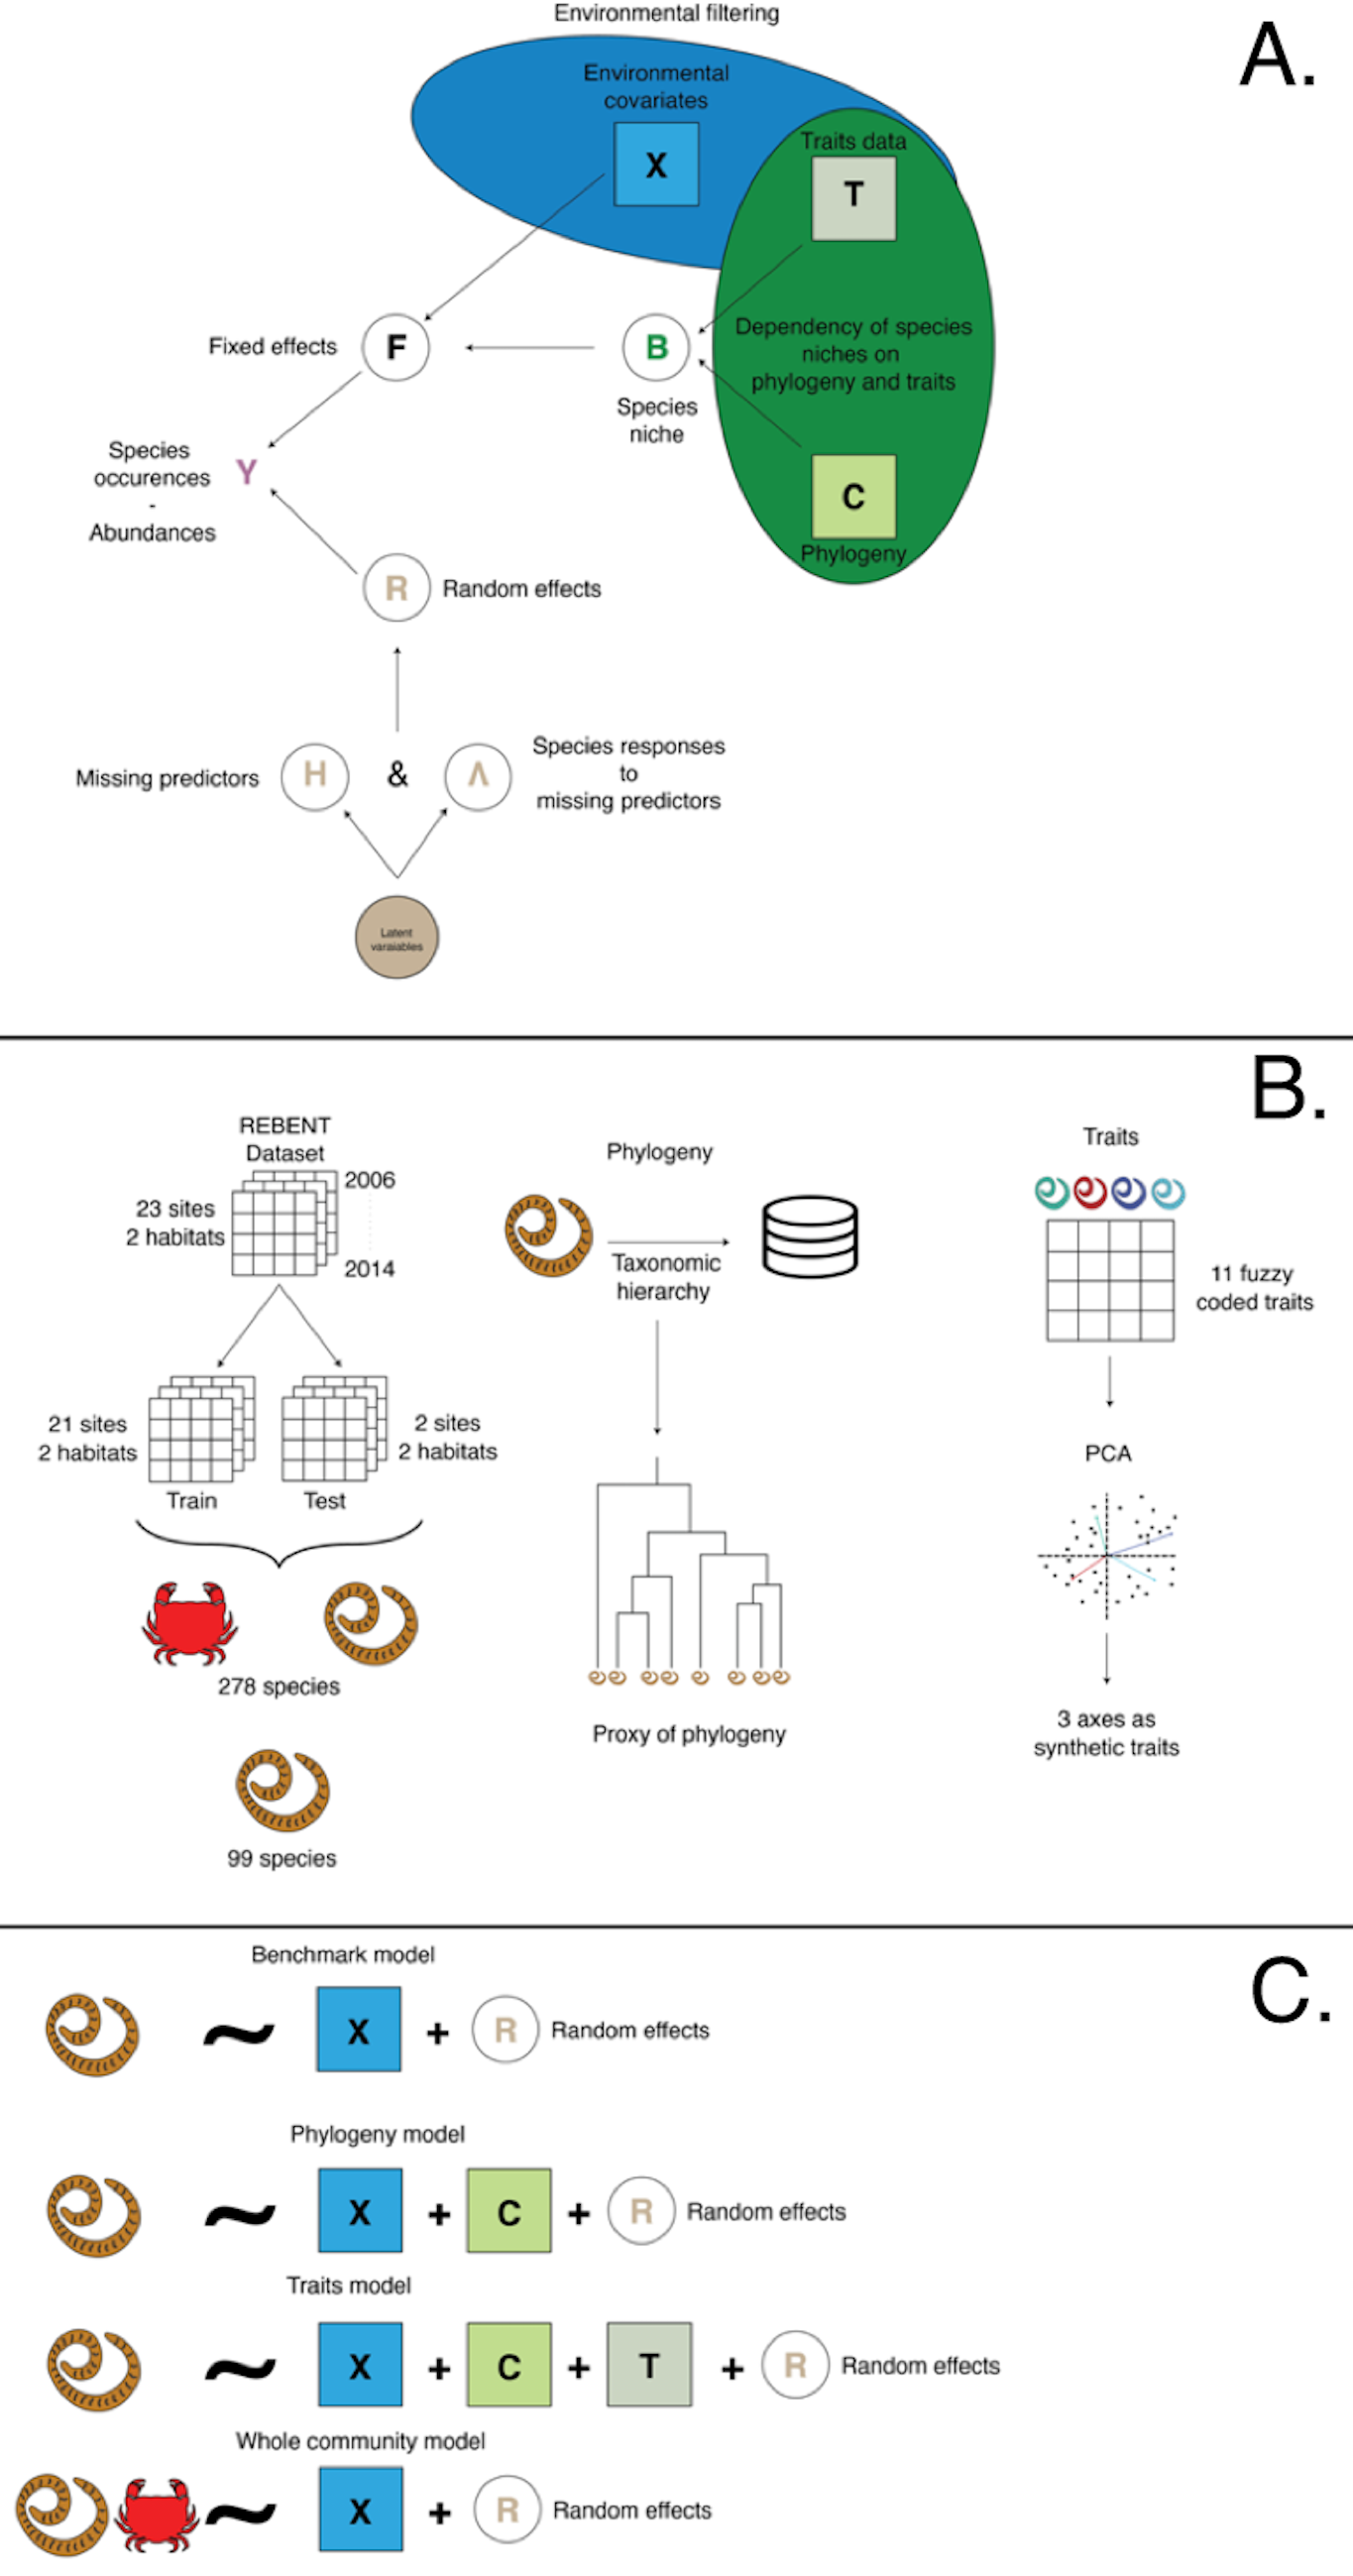
\includegraphics{figures/fig1.png}
\caption{Study workflow. A. \emph{Hierarchical Model of Species
Community} (\emph{HMSC}) structure, incorporating environmental
variables, phylogeny, and species-specific traits. B. Data
pre-processing: partitioning community data into train and test
datasets, estimating phylogenetic distance (using taxonomic
classification), and dimension reduction of species-trait matrix using
fuzzy-PCA. C. Summary of the four alternative model structures fitted to
presence/absence and abundance data: the \emph{Bench}mark, Phylogeny,
Traits \& Phylogeny models only consider the targeted polychaetes, while
the Whole Community model includes additional species potentially
interacting with the target assemblage. Random effects for sampling
year, site, and habitat were included in all
models.}\label{fig:chapt1workflow}
}
\end{figure}

\hypertarget{datasets}{%
\subsection{Datasets}\label{datasets}}

\hypertarget{faunistic-data}{%
\subsubsection{Faunistic data}\label{faunistic-data}}

The \emph{REBENT} program
(\href{https://rebent.ifremer.fr}{rebent.ifremer.fr}) is an ongoing
monitoring of benthic macrofauna across multiple stations along
Brittany's coastline (Western France). Here, we used data from
\textcite{Boye_2019a}, covering 23 sites and two intertidal soft-bottom
habitats: bare sands and seagrass meadows (Fig. S1) where infaunal
communities were monitored yearly using the same protocol between 2006
and 2014. A detailed description of the sampling methodology is provided
in \autocites[ ]{Boye_2017}{Boye_2019a}. At each site, three faunal
samples (0.03 m\(^2\) cores) were taken at each of three fixed sampling
points distributed 200 m apart. These samples were then pooled together
to estimate abundances at the site level. For each sampling event,
individuals were identified to the lowest taxonomic level possible
(mostly species level; for simplicity we hereafter refer to
``species'').

Overall, across a total of 375 sampling units (i.e.~unique combination
of years, sites and habitats), 152,583 individuals belonging to 519
species were collected and identified. To avoid convergence issues and
poor model inference, we filtered out species occurring less than four
times (across the 180 samples used as train set, see below), resulting
in the removal of 241 species. The remaining 278 species included 99
polychaete species (the targeted assemblage) and 179 non-target species
of bivalves, molluscs, and amphipoda, which may predate or compete with
polychaetes \autocites[ ]{Grall_2006}{Jankowska_2019}. We chose to focus
on polychaetes as this taxonomic group exhibits diverse lifestyles
\autocite{Jumars_2015}, can be used to monitor the health of benthic
habitats \autocite{Giangrande_2005}, and because trait data and
ecological information were available from previous studies
\autocite{Boye_2019a}.

\hypertarget{traits-and-phylogeny-data}{%
\subsubsection{Traits and phylogeny
data}\label{traits-and-phylogeny-data}}

Traits data were retrieved from \autocite{Boye_2019a} for the 99
polychaete species present in the train set (see below). The 11
fuzzy-coded traits available (see \textcite{Boye_2019a} for details)
were synthetized using a fuzzy-PCA, with the \emph{fpca} function from
the \emph{ade4} R package \autocite{Thioulouse_2018}. The first three
axes, which account for 59\% of the total variance of the trait matrix,
were included in the model as synthetic traits data
(fig.~\ref{fig:chapt1workflow}). The first axis distinguishes mobile
predatory species from sessile microphages; the second axis
differentiates semelparous species from iteroparous species; and, the
third axis separates burrowers from tube-dwellers (Fig. S2).

Phylogeny was not available, hence we followed common practices
\autocite{Ovaskainen_2020} and retrieved the taxonomic classification of
these 99 polychaetes through the WoRMS database
(\href{https://www.marinespecies.org}{www.marinespecies.org}; january
2020) and used this information as a proxy for phylogenetic
relationships (fig.~\ref{fig:chapt1workflow} ;
\textcite{Ovaskainen_2020}). Phylogenetic distances were then estimated
using the ape R package \autocite{Paradis_2019}.

\hypertarget{environmental-data}{%
\subsubsection{Environmental data}\label{environmental-data}}

Following \textcite{Boye_2019a} (see Appendix A for details about data
sources), we selected seven environmental variables to characterise the
ecological niche of each species. These seven variables quantify
different components of coastal environmental variability including
hydrology (sea water temperature, salinity and current velocity),
sedimentology (mud and organic matter content), substrate heterogeneity
(Trask index) and local wave exposure (fetch). For each of these seven
variables, the first- and second-degree polynomials were computed to
account for non-linear responses.

\hypertarget{comparison-of-alternative-model-structures}{%
\subsection{Comparison of alternative model
structures}\label{comparison-of-alternative-model-structures}}

The first model (denoted \emph{Bench}) only considers data for the 99
target polychaete species and the 7 environmental covariates
(fig.~\ref{fig:chapt1workflow}). The second model (denoted \emph{Ph})
adds phylogenetic data to the \emph{Bench} model
(fig.~\ref{fig:chapt1workflow}). The third model (denoted \emph{TrPh})
adds traits data to the \emph{Ph} model. The fourth model (denoted
\emph{WhC}) has the same structure as the \emph{Bench} model but
includes data on the whole community (278 species, including 179
additional non-target species; fig.~\ref{fig:chapt1workflow}).
\emph{WhC} excludes traits (unavailable for the non-target taxa) and
phylogenetic data for faster computation. Each model was fitted twice,
either with presence/absence or abundance data, using probit and
lognormal Poisson distributions respectively. All models include the
same random effects (fig.~\ref{fig:chapt1workflow}): temporal, spatial
(sites), and habitats (bare vs seagrass).

\hypertarget{model-fitting}{%
\subsection{Model fitting}\label{model-fitting}}

We estimated model parameters by running 5 chains using a MCMC sampling
algorithm over 375,000 iterations. The first 125,000 iterations were
discarded as burn-in while the remaining were thinned every 250
iterations yielding 1,000 posterior samples per chain for an overall
total of 5,000 posterior samples for each parameter. We assessed
convergence for each model parameter using both potential scale
reduction factor \autocite{Gelman_1992} and effective sample size as
reported in supplementary materials (Appendix B). All models were fitted
using the DATARMOR supercomputing facility.

\hypertarget{assessing-model-performance-and-interpretability}{%
\subsection{Assessing model performance and
interpretability}\label{assessing-model-performance-and-interpretability}}

For independent assessment of models' predictive performance, the
dataset was split into a train and a test set, instead of using strict
cross-validation procedure that would have considerably increase the
computational burden (see also \textcite{Norberg_2019}). The train
dataset consisted of 180 sampling units (21 sites; one or two habitats,
and six to nine years per site; Fig. S1). The test set comprised 35
sampling units covering a 9-year period at two specific sites with both
seagrass and bare sand habitats. These sites were chosen as
representative of both regional macrofaunal species diversity (all the
species observed in the test set are also observed in the train set) and
mean environmental conditions (which limits model extrapolation outside
of the trained parameter space; Fig. S3-S4; \textcite{Boye_2017} ;
\textcite{Boye_2022} ; \textcite{Toumi_2023}).

To assess \emph{jSDM's} performance, we used a set of complementary
metrics to evaluate both their explanatory and predictive abilities on
the train and test dataset, respectively (Table 1). AUC and RMSE,
calculated only for the 99 target species (i.e.~polychaetes) even for
the \emph{WhC} model that includes a total of 278 species, were used to
assess overall and species-level performance for presence/absence and
abundance models, respectively. Relationships between observed and
predicted mean species abundances across all sites were also visualized
for abundance models.

Along with the raw AUC and RMSE values, we also visualized and
quantified changes relative to the \emph{Bench} model for the \emph{Ph},
\emph{TrPh} and \emph{WhC} models. For abundance models, we computed the
overall relative change in mean RMSE across species as:

\begin{equation}\protect\hypertarget{eq:eq1}{}{\text{Relative change} = \frac{\text{mean}\left(\text{RMSE}_{\text{ focal model}}\right) - \text{mean}\left(\text{RMSE}_{\text{Bench}}\right)}{\text{mean}\left(\text{RMSE}_{\text{Bench}}\right)} \times 100}\label{eq:eq1}\end{equation}

AUC and RMSE only partially capture model accuracy at the community
scale (Table 1). To explore this aspect, we focused on differences
between predicted and observed assemblage richness and total abundances
(for abundance models). We also compared observed and predicted Sørensen
(for presence/absence) and Bray-Curtis (abundance)
pairwise-dissimilarity matrices to explore how well \(\beta\)-diversity
patterns were reproduced by the models. For these three metrics, we
computed relative change for both the train and test datasets between
mean predicted and mean observed values as follows:

\begin{equation}\protect\hypertarget{eq:eq2}{}{\text{Relative change} = \frac{\text{mean}\left(\text{Metric}_{\text{ predict}}\right) - \text{mean}\left(\text{Metric}_{\text{ obs}}\right)}{\text{mean}\left(\text{Metric}_{\text{ obs}}\right)} \times 100}\label{eq:eq2}\end{equation}

where ``Metric'' is a community-based measure (e.g.~species richness,
total abundance, dissimilarity matrices) estimated from model
predictions or observations at the sample level (i.e.~unique combination
of site, habitat and year; or, pairs of samples for dissimilarity). To
evaluate model interpretability, we calculated the amount of explained
variance per species and the proportion that can be attributed to
environmental covariates (fixed effects) and random effects. We compared
the overall relative change in the proportion of variance explained by
the covariates and by the random effects for the \emph{Ph}, \emph{TrPh}
and \emph{WhC} relative to the \emph{Bench} model (by comparing mean
values across species similarly to eq.~\ref{eq:eq1}). We also propose a
novel way of exploring species-environment relationships (Table 1) by
classifying the response curves estimated from the different models
based on their shapes, considering both their direction (decline, null,
or increase) and their acceleration (decelerated, constant, or
accelerated) \autocite{Rigal_2020}. Finally, we compared the residual
co-occurrence patterns associated with each random effect of the
\emph{Bench} model with those of the best performing model (\emph{WhC}).
We quantified differences in magnitude and sign of residual
species-species correlations using the following index:

\begin{equation}\protect\hypertarget{eq:eq3}{}{\delta = |corr_{\text{ best model}} - corr_{\text{ Benchmark}}| \times sign(corr_{\text{ best model}} \times corr_{\text{ Benchmark}})}\label{eq:eq3}\end{equation}

\clearpage
\thispagestyle{empty}
\newgeometry{margin=1.25cm}
\begin{landscape}

% Otherwise, the font cite of the command citation is normal
\renewcommand*{\citesetup}{\scriptsize}

\begin{table}[htbp]
\caption[Multi-assessment framework providing a list of metrics to assess, interpret or compare jSDMs across different ecological facets at the species, community or overall level.]{\footnotesize Multi-assessment framework providing a list of useful metrics to assess, interpret or compare jSDMs across different ecological facets (rows) at the species, community or overall level. Italicized metrics are used in this study.}
    \begin{threeparttable}
    \begin{scriptsize}
    \begin{tabular}{ccccccc}
        \multicolumn{2}{|c|}{Model outputs} & \multicolumn{1}{c|}{\shortstack[c]{Example of derived-metrics\\for model interpretation}} & \multicolumn{2}{c|}{\shortstack[c]{Example of derived-metrics\\for model evaluation}} & \multicolumn{2}{c|}{\shortstack[c]{Example of performance measures\\to assess the explanatory/predictive\\power of models\footnotemark}} \\
        \cline{4-7}
        \multicolumn{2}{|c|}{} & \multicolumn{1}{c|}{} & \multicolumn{1}{c|}{Presence/Absence} & \multicolumn{1}{c|}{Abundance} & \multicolumn{1}{c|}{Presence/Absence} & \multicolumn{1}{c|}{Abundance} \\
        \hline\hline
        \multicolumn{1}{|c|}{Species level} & \multicolumn{1}{c|}{\shortstack[c]{Abundance,\\occurrence probability,\\environmental coefficients}} & \multicolumn{1}{c|}{\shortstack[c]{Variable importance (e.g. LIME, SHAP\footnotemark),\\Heatmap of environmental coefficients,\\ \emph{Response curves}\footnotemark, \emph{Variance partitioning}}} & \multicolumn{1}{c|}{\shortstack[c]{Number of\\Presence/Absence,\\Proportion of\\occupied sites}} & \multicolumn{1}{c|}{\shortstack[c]{Total abundance,\\site-specific\\abundance}} & \multicolumn{1}{c|}{\shortstack[c]{\emph{AUC},\\Kappa,\\F1-Score}} & \multicolumn{1}{c|}{\shortstack[c]{\emph{RMSE}, MAE, R2,\\Correlation between\\predicted and\\observed values}} \\
        \hline
        \multicolumn{1}{|c|}{$\alpha$-diversity} & \multicolumn{1}{c|}{\multirow{2}{*}{\shortstack[c]{Site-specific community\\composition}}} & \multicolumn{3}{c|}{\shortstack[c]{Diversity index (e.g. Shannon entropy,\\Simpson-Gini index), \emph{Total abundance},\\\emph{Total richness},\\Proportion of rare/abundant species}} & \multicolumn{2}{c|}{\multirow{2}{*}{\shortstack[c]{\emph{Differences between predicted and observed values},\\RMSE, MAE, R2,\\Correlations (e.g. Kendall, Pearson)\\between observed and predicted\\alpha or beta diversity indices}}} \\
        \cline{1-1}\cline{3-5}
        \multicolumn{1}{|c|}{$\beta$-diversity} & \multicolumn{1}{c|}{} & \multicolumn{3}{c|}{\shortstack[c]{\emph{Pairwise dissimilarity} (e.g. Jaccard/Bray-Curtis),\footnotemark\textsuperscript{,}\footnotemark\\Total Beta diversity, Turnover,Nestedness,\\Local Contribution to Beta Diversity (LCBD),\\Species Contribution to Beta Diversity (SCBD)}} & & \multicolumn{1}{c|}{} \\
        \hline
        \multicolumn{1}{|c|}{\multirow{3}{*}{\shortstack[c]{Overall\\assessment\\(all sites)}}} & \multicolumn{1}{c|}{\shortstack[c]{Regional community\\composition}} & \multicolumn{3}{c|}{\shortstack[c]{Diversity index (e.g. Shannon entropy,\\Simpson-Gini index), Total abundance,\\Total richness,\\Proportion of rare/abundant species}} & \multicolumn{1}{c|}{\shortstack[c]{Average over all species:\\\emph{AUC}, Kappa, F1-Score}} & \multicolumn{1}{|c|}{\shortstack[c]{Average over all species:\\\emph{RMSE}, MAE, R2,\\Correlation \emph{between predicted}\\\emph{and observed values}}} \\
        \cline{2-7}
        \multicolumn{1}{|c|}{} & \multicolumn{1}{c|}{\shortstack[c]{Residual correlation\\matrix}} & \multicolumn{1}{c|}{\shortstack[c]{Co-occurrence network\\analysis (e.g centrality,\\number of degrees)}} & \multicolumn{4}{c|}{\shortstack[c]{Comparison with observed or reconstructed networks\\(expert-based or estimated e.g. based on trophic analyses) ,\\using e.g. correlations, \emph{residual correlation index ($\delta$)}\footnotemark}} \\
        \cline{2-7}
        \multicolumn{1}{|c|}{} & \multicolumn{1}{c|}{\shortstack[c]{Trait-based\\regression coefficients}} & \multicolumn{1}{c|}{\shortstack[c]{\emph{Traits-environment}\\\emph{response curves}, Heatmap\\of traits-environment coefficients}} & \multicolumn{4}{c|}{\shortstack[c]{Qualitatively, based on\\literature and/or\\expert knowledge\footnotemark}} \\
        \hline
    \end{tabular}
    \par\noindent\rule{\textwidth}{0.5pt}
    \vspace{\baselineskip}
    \end{scriptsize}
    \begin{tablenotes}
        \scriptsize
        \item[1] All performance measures can theoretically be compared between models. For instance, we here measured differences between models using a measure of relative change in RMSE or AUC relative to the Bench model using Eq. 1. Other measures could be correlations between model predictions.
        \item[2] See \textcite{Ryo_2021}
        \item[3] To ease model comparison and interpretation, we propose to summarize the information contained in species response curves using the framework initially proposed by \textcite{Rigal_2020} for classifying species temporal trajectories based on their trend, acceleration, direction and velocity. Applied to regression coefficients, it allows to classify the response of species to each environmental variable into several shapes that are easy to interpret, to link with ecological theory, and to compare across models.
        \item[4] For jSDM assessment, pairwise dissimilarities can be computed on the observed site-by-species matrix and on the predicted one. Comparing these values (e.g. through correlation analysis or simply through differences) will inform on how well the model reproduces/predict beta diversity patterns. Alternatively, pairwise dissimilarities can be computed between the observed taxa composition of a sample and its predicted one. These dissimilarities then become a metric to assess model performance based on species-composition predictions.
        \item[5] For jSDMs comparisons, pairwise dissimilarities computed between the observed taxa composition of a sample and its predicted one can be compared across models (e.g. through correlations) to assess to what extent differences between predicted and observed taxa composition are congruent across different models. Alternatively, comparing correlations between pairwise dissimilarities computed on the observed site-by-species matrix and on the predicted one will inform on which model best predict beta diversity patterns.
        \item[6] Species interaction networks can be reconstructed under certain conditions using the residual correlation matrices estimated by jSDM (see \textcite{Momal_2020}). The comparison between these reconstructed interaction networks and already known interaction networks (based on trophic data, experimental data, expert knowledge or qualitative information on species interactions) can serve as a means of model validation.
        \item[7] Comparing modelled species trait-environment responses (e.g., signs, shape of response curves) with expected responses (e.g. from theory, experiments or expert knowledge) can also serve to validate qualitatively the models.
    \end{tablenotes}
    \end{threeparttable}
\end{table}
\end{landscape}
\label{tbl1}
\restoregeometry



\hypertarget{results}{%
\section{Results}\label{results}}

Both MCMC convergence and effective sample size of the different
\emph{jSDMs} were satisfactory (see Appendix D).

\hypertarget{model-fit-predictive-power}{%
\subsection{Model Fit \& Predictive
power}\label{model-fit-predictive-power}}

\hypertarget{species-level}{%
\subsubsection{Species level}\label{species-level}}

Presence/absence models showed excellent explanatory power with mean
AUCs above 0.9 on the train dataset, but lower predictive power with
mean AUCs around 0.66 on the test set (Fig. S17). Both explanatory (mean
AUC between 0.92 and 0.93) and predictive (mean AUC between 0.64 and
0.66) power were overall similar across models
(fig.~\ref{fig:chapt1fig2}, Fig. S17). Within the target species
assemblage, predictions improved for 41 species and worsened for 36
species (out of the 99 target species, which implies marginal changes
for the remaining 22) in the \emph{WhC} model relative to the benchmark.
In comparison in the \emph{Ph} or the \emph{TrPh} models, predictions
only improved for 26 and 27 species, respectively, and worsened for 49
and 48 species, respectively.

Abundance models also showed a satisfactory explanatory power with a
mean RMSE close to nine for all models, given a mean abundance in the
train dataset of 307.31 ± 583.58 (mean ± sd). Overall, all models
underpredicted species abundances (Fig. S18-19). While explanatory power
was similar across models, larger variations were observed for
predictive power. The \emph{Bench} model had a mean RMSE of 126.67 (for
a mean abundance in the test dataset of 700.57 ± 818.66; Fig S17). The
Ph model performed better (mean RMSE of 62.23; -50.87\% compared to the
\emph{Bench}; Fig. S17) whereas the \emph{TrPh} model did worse (mean
RMSE of 139.21; +9.90\%; Fig. S17). The best model was the \emph{WhC}
with a mean RMSE of 6.59 (-94.80\% compared to the \emph{Bench}, Fig.
S17). Out of the 99 target species, the \emph{WhC} model predictions
improved for 57 species but declined for 15 species relative to the
Bench. Conversely, performance gain for the \emph{Ph} and \emph{TrPh}
models were poor relative to the Bench, as predictions improved for 38
and 31 species, respectively, but declined for 40 and 46 species,
respectively.

We further investigated this gain in predictive power of the \emph{WhC}
model fitted to abundance data by examining the relationships between
changes in predictive power and the occurrence or abundance of the
species. On the test set, performance of the \emph{WhC} model most
improved relative to the \emph{Bench} model for rare species
(correlation with average species abundance: Kendall's \(\tau = 0.12\),
\(\text{p-value} < 0.05\); Fig. S20). However, we found no patterns
between change in RMSE relative to the Bench model and proportion of
presence (Kendall's \(τ\tau = 0.12\), \(\text{p-value} = 0.09\); Fig
S21).

\begin{figure}
\hypertarget{fig:chapt1fig2}{%
\centering
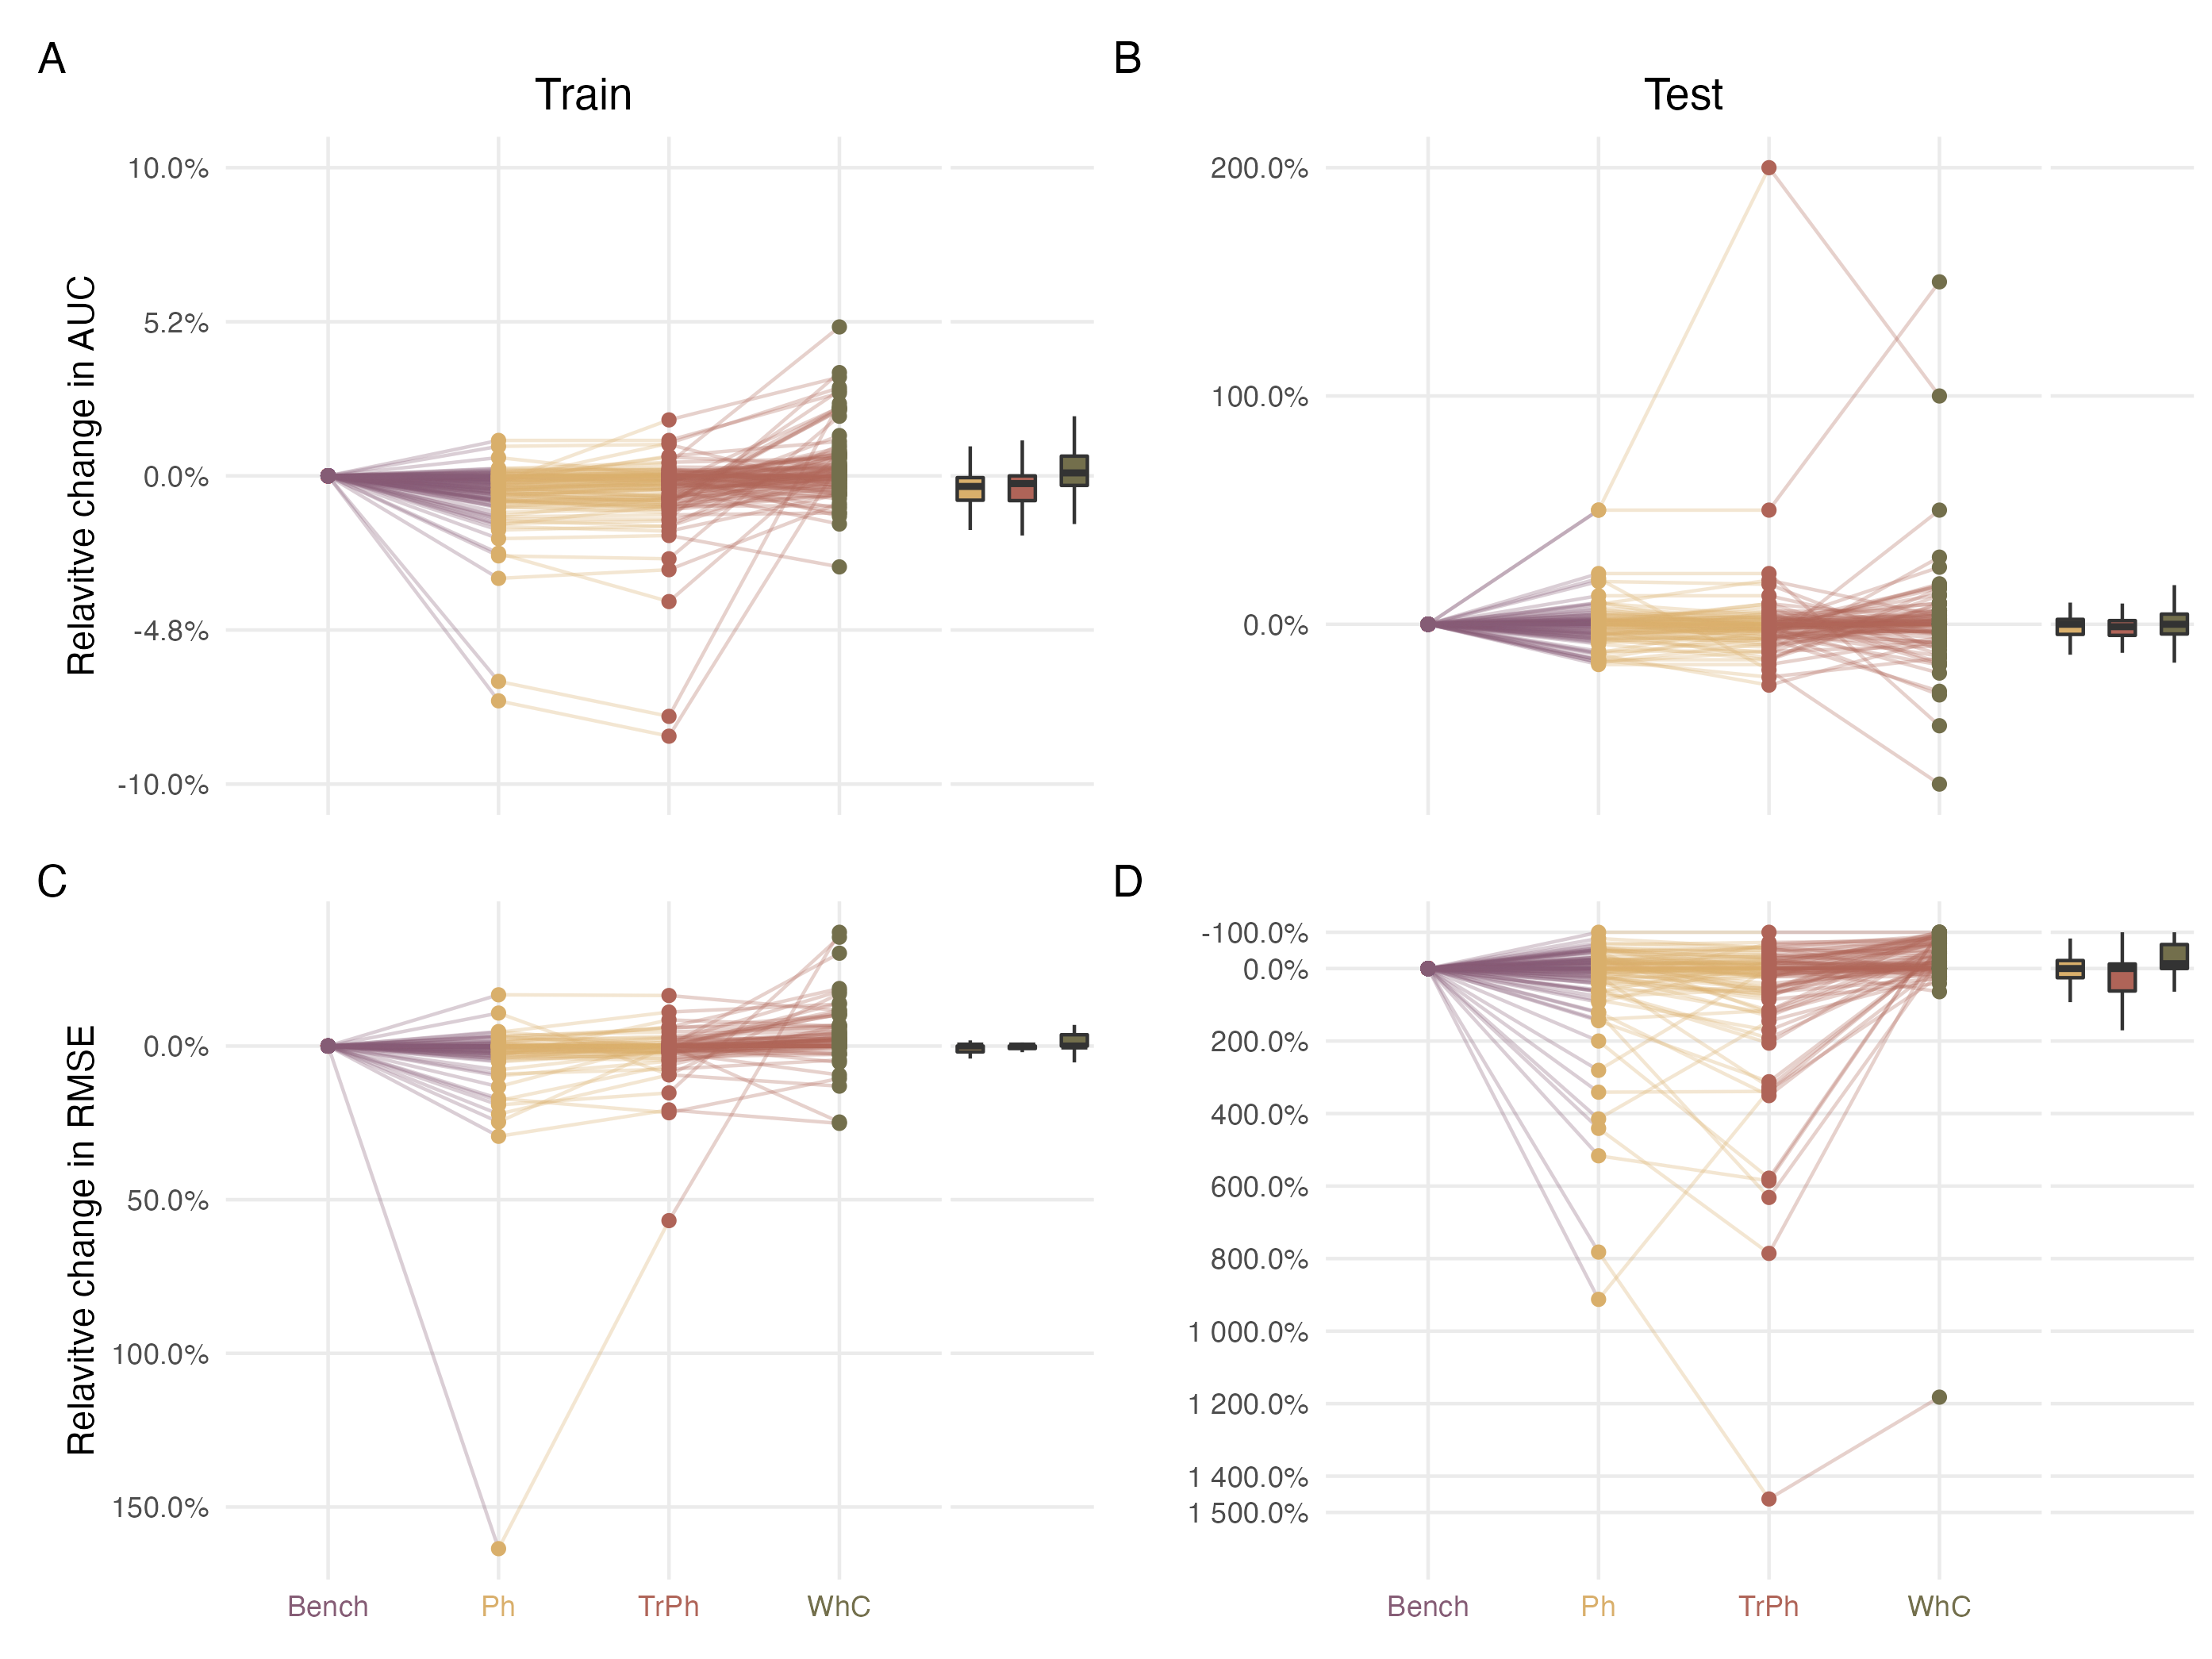
\includegraphics{figures/fig2.png}
\caption{Change in explanatory and predictive power of three model
structures (yellow for \emph{Phylogeny} (\emph{Ph}), red for
\emph{Traits and phylogeny} (\emph{TrPh}), and green for \emph{Whole
community} (\emph{WhC}) models) relative to the \emph{Benchmark model}
(\emph{Bench}; purple). Changes are expressed as percentages relative to
the benchmark fitted on presence/absence (top row) or abundance (bottom
row) data. Points above the zero line indicate performance
gain.}\label{fig:chapt1fig2}
}
\end{figure}

\hypertarget{community-level}{%
\subsubsection{Community level}\label{community-level}}

In terms of alpha diversity, the \emph{Bench}, the \emph{Ph} and
\emph{TrPh} models fitted on abundance data all underpredicted mean
species richness of the train set by 4 species on average (-29.2\%
compared to observed data; fig.~\ref{fig:chapt1fig3}). In contrast, the
\emph{WhC} model overpredicted mean richness by 11 species on average
(+80\% compared with observed data). Similar results were found on the
test dataset with the \emph{Bench}, \emph{Ph} and \emph{TrPh} models
underpredicting richness by 5 species (-24.9 \%) on average whereas the
\emph{WhC} model overpredicted richness by 7 species (+35.8\% compared
with observed data). Similar results were found for models fitted on
presence/absence data (Fig. S22).

All models overall underpredicted mean total abundance relative to the
train dataset (fig.~\ref{fig:chapt1fig3}), by 153 individuals for the
\emph{Bench} model (-49.8\% compared to observed data) and by 159 and
155 individuals (-51.7\% and -50.4\%) for the \emph{Ph} and \emph{TrPh}
models, respectively. The \emph{WhC} model only underpredicted total
abundance by 22 individuals (-7.12\% compared to observed data).
Relative to the test dataset, the \emph{Bench}, the \emph{Ph} and the
\emph{TrPh} models overpredicted mean total abundance by 1642 (+234\%
compared to observations), 465 (+66.3\%), and 1969 individuals (+281\%),
respectively. In contrast, the \emph{WhC} model underpredicted mean
total abundance of the test data samples by 404 individuals on average
(-57.6\%).

Mean beta diversity patterns in the train dataset were overall well
captured by all models fitted on abundance or presence/absence data
(fig.~\ref{fig:chapt1fig3}). Observed dissimilarities were slightly
overpredicted by all abundance models: by 0.057 for the \emph{Bench}
(+7.3\% compared with observed data), 0.050 for the \emph{Ph} (+6.4\%),
0.054 for the \emph{TrPh} (+6.9\%) and 0.070 for the \emph{WhC} models
(+8.9\%). Differences for presence/absence models were of similar order
but all models underpredicted mean pairwise dissimilarities between
samples (Fig. S22). On the test dataset, beta diversity patterns were
rather poorly captured by the models fitted on abundance data. The Bench
model overpredicted the pairwise dissimilarities by 0.364 on average
(+67.1\% compared with observed data), the \emph{Ph} model by 0.365
(+67.4\%), the \emph{TrPh} model by 0.375 (+69.1\%) and the \emph{WhC}
model by 0.338 (+62.4\%). Similar results were observed for
presence/absence models with slightly smaller overpredictions (Fig.
S22).

\begin{figure}
\hypertarget{fig:chapt1fig3}{%
\centering
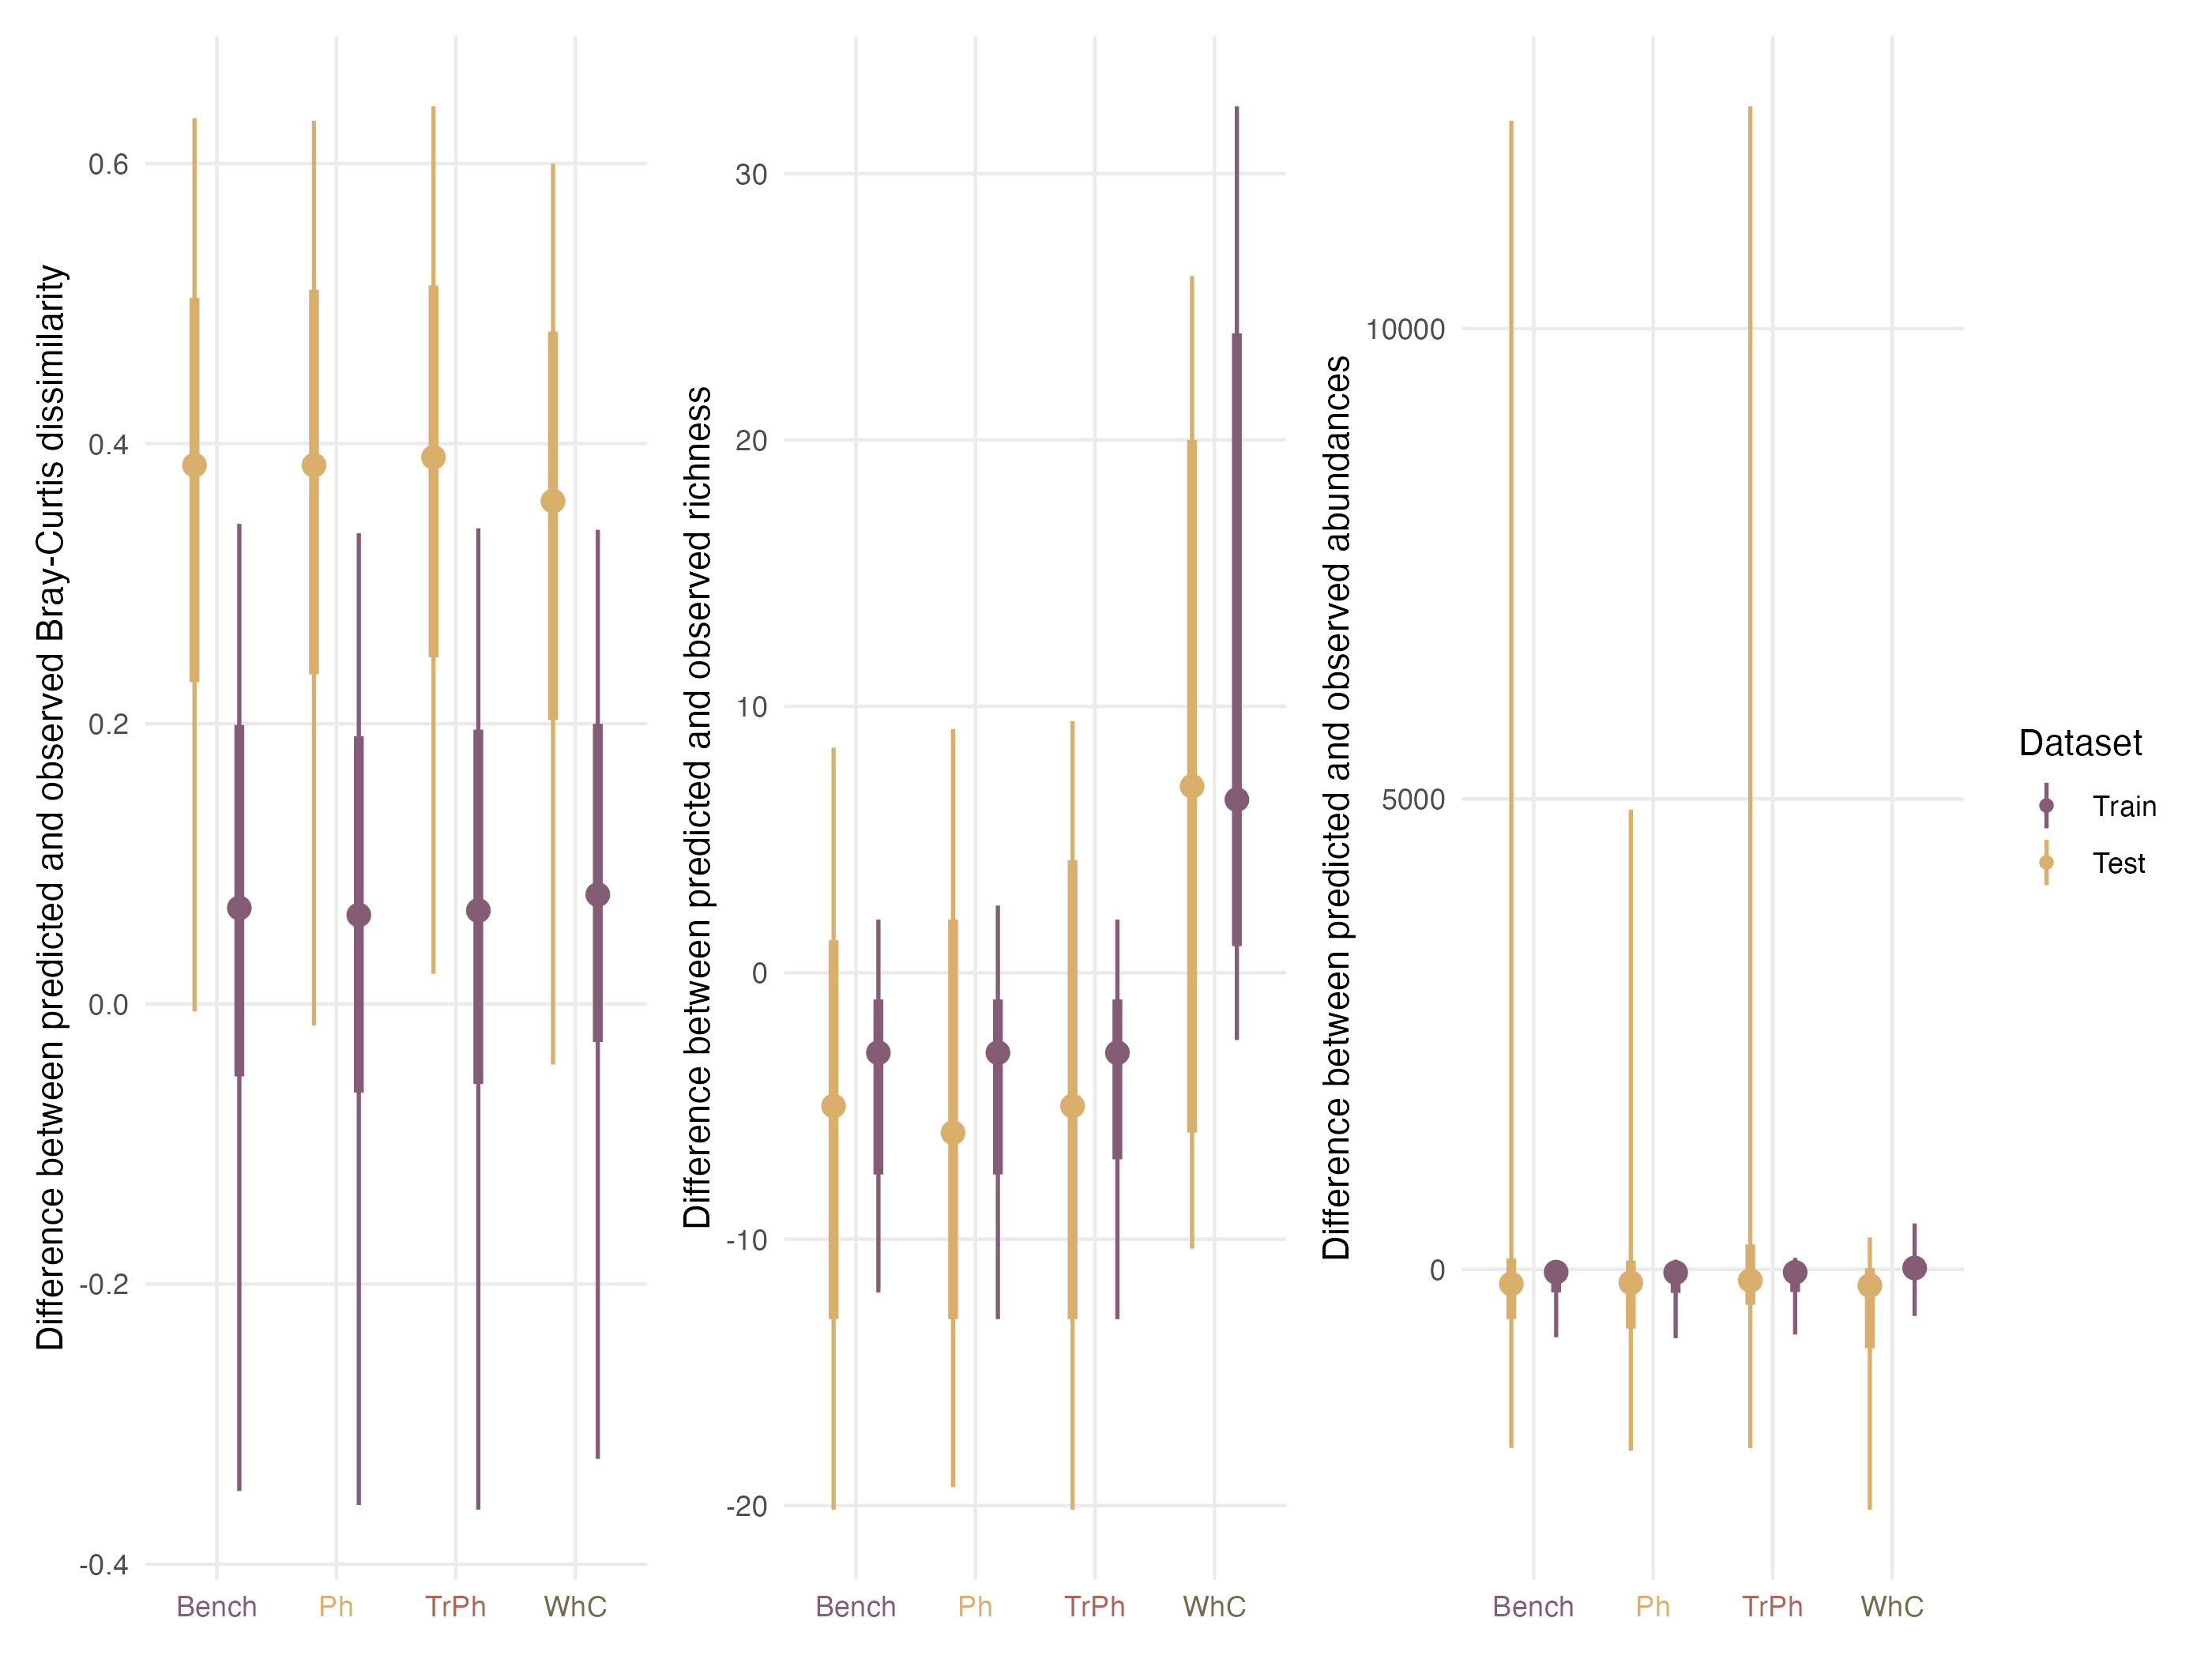
\includegraphics{figures/fig3.png}
\caption{Comparison of model performances with regards to their ability
to predict community structures when fitted with abundance data for the
train (purple) and test (yellow) dataset. Left: differences in pairwise
dissimilarities estimated on the observed and the predicted assemblages.
Centre: differences in species richness between observed and predicted
assemblages. Right: differences in total abundance between observed and
predicted assemblages.}\label{fig:chapt1fig3}
}
\end{figure}

\hypertarget{variance-partitioning}{%
\subsection{Variance partitioning}\label{variance-partitioning}}

The mean amount of total variance explained across the 99 polychaetes
varied between 21 and 23\% for models fitted with presence/absence data
and between 18 and 30\% for abundance-based models (Fig. S23). For all
models, environmental variables, rather than random effects, accounted
for most (more than 68\% ± 18\%; mean ± s.d.) of the explained variance
(Fig. S24). However, a larger part of variance is explained by random
effects in the \emph{WhC} model compared to the other models, including
the Bench (Fig. S24). Compared to the \emph{Bench} model fitted with
abundance data, the relative change in the part of variance explained by
random effects across the 99 species decreased by 17.00\% for the
\emph{Ph} model, 10.90\% for the \emph{TrPh} model and increased by
224\% for the \emph{WhC} model (fig.~\ref{fig:chapt1fig4}). Similar
results with smaller relative changes were obtained across
presence/absence models (fig.~\ref{fig:chapt1fig4} ; Fig. S23-24).

\begin{figure}
\hypertarget{fig:chapt1fig4}{%
\centering
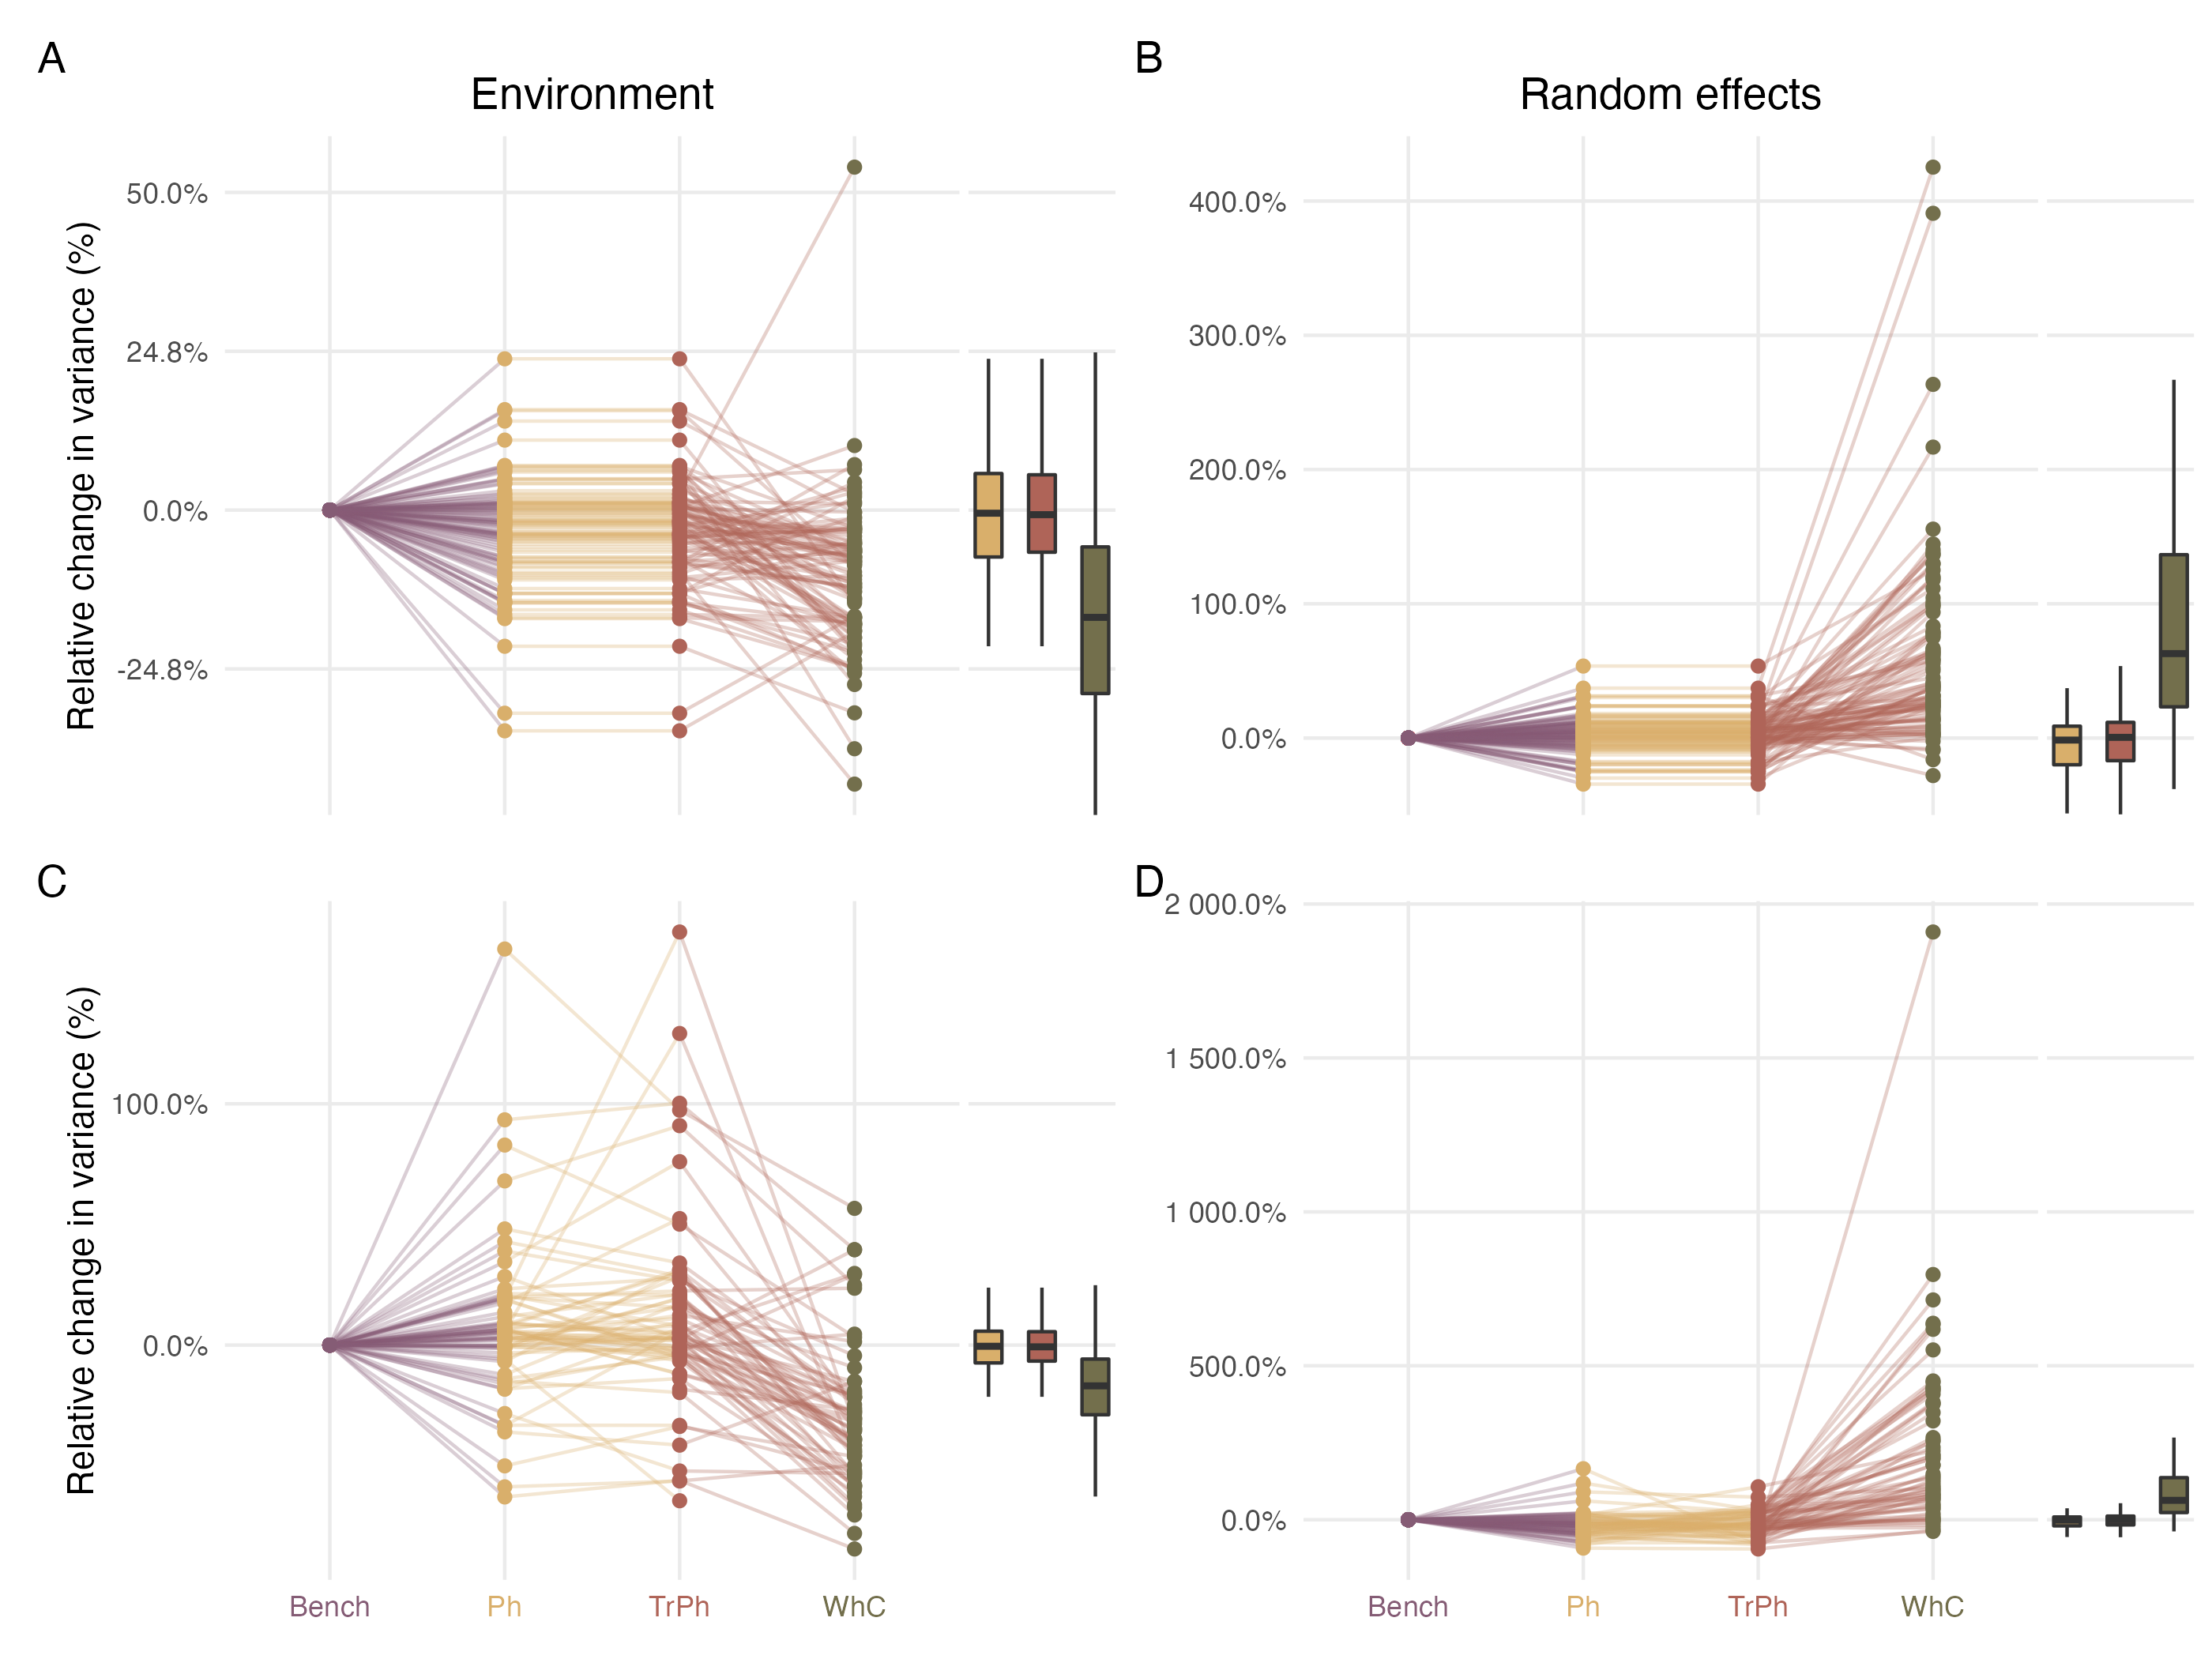
\includegraphics{figures/fig4.png}
\caption{Change in explained variance related to environmental
predictors (left column) and random effects (right column) for three
alternative model structures (yellow for \emph{Phylogeny} (\emph{Ph}),
red for \emph{Traits and phylogeny} (\emph{TrPh}), and green for
\emph{Whole community} (\emph{WhC}) models) relative to the
\emph{Benchmark model} (\emph{Bench}; purple). Percentage changes were
computed relative to the \emph{Benchmark model} fitted with
presence/absence (top panels) or abundance (bottom panels) data.
Positive values indicate an increase in the proportion of variance
explained by the focal model compared to the \emph{Benchmark model}. See
Figure S23 and S24 for the raw percentages, expressed as percentages of
explained variance or total amount of variance
respectively.}\label{fig:chapt1fig4}
}
\end{figure}

\hypertarget{species-niche-estimated}{%
\subsection{Species niche estimated}\label{species-niche-estimated}}

For abundance models, the large majority (\textgreater60\%) of flat
response curves indicated a lack of meaningful species-environment
relationships (fig.~\ref{fig:chapt1fig5}). This proportion reached 83\%
for the \emph{WhC} model. The prevalence of flat relationships did not
appear to be related to convergence issues (Fig. S15-16) or to be driven
by a specific covariate (Fig. S25). Convex or concave response curves
were rare in abundance models. Significant relationships primarily
included constant or accelerated declines, representing approximately
10\% and 15\% of response curves in the \emph{Bench}, \emph{TrPh}, and
\emph{Ph} models (fig.~\ref{fig:chapt1fig5}). In the \emph{WhC} model,
these percentages decreased to 7\% and 6\%, respectively
(fig.~\ref{fig:chapt1fig5}). Similar findings were observed for
presence/absence models (Fig. S26; Fig. S27).

\begin{figure}
\hypertarget{fig:chapt1fig5}{%
\centering
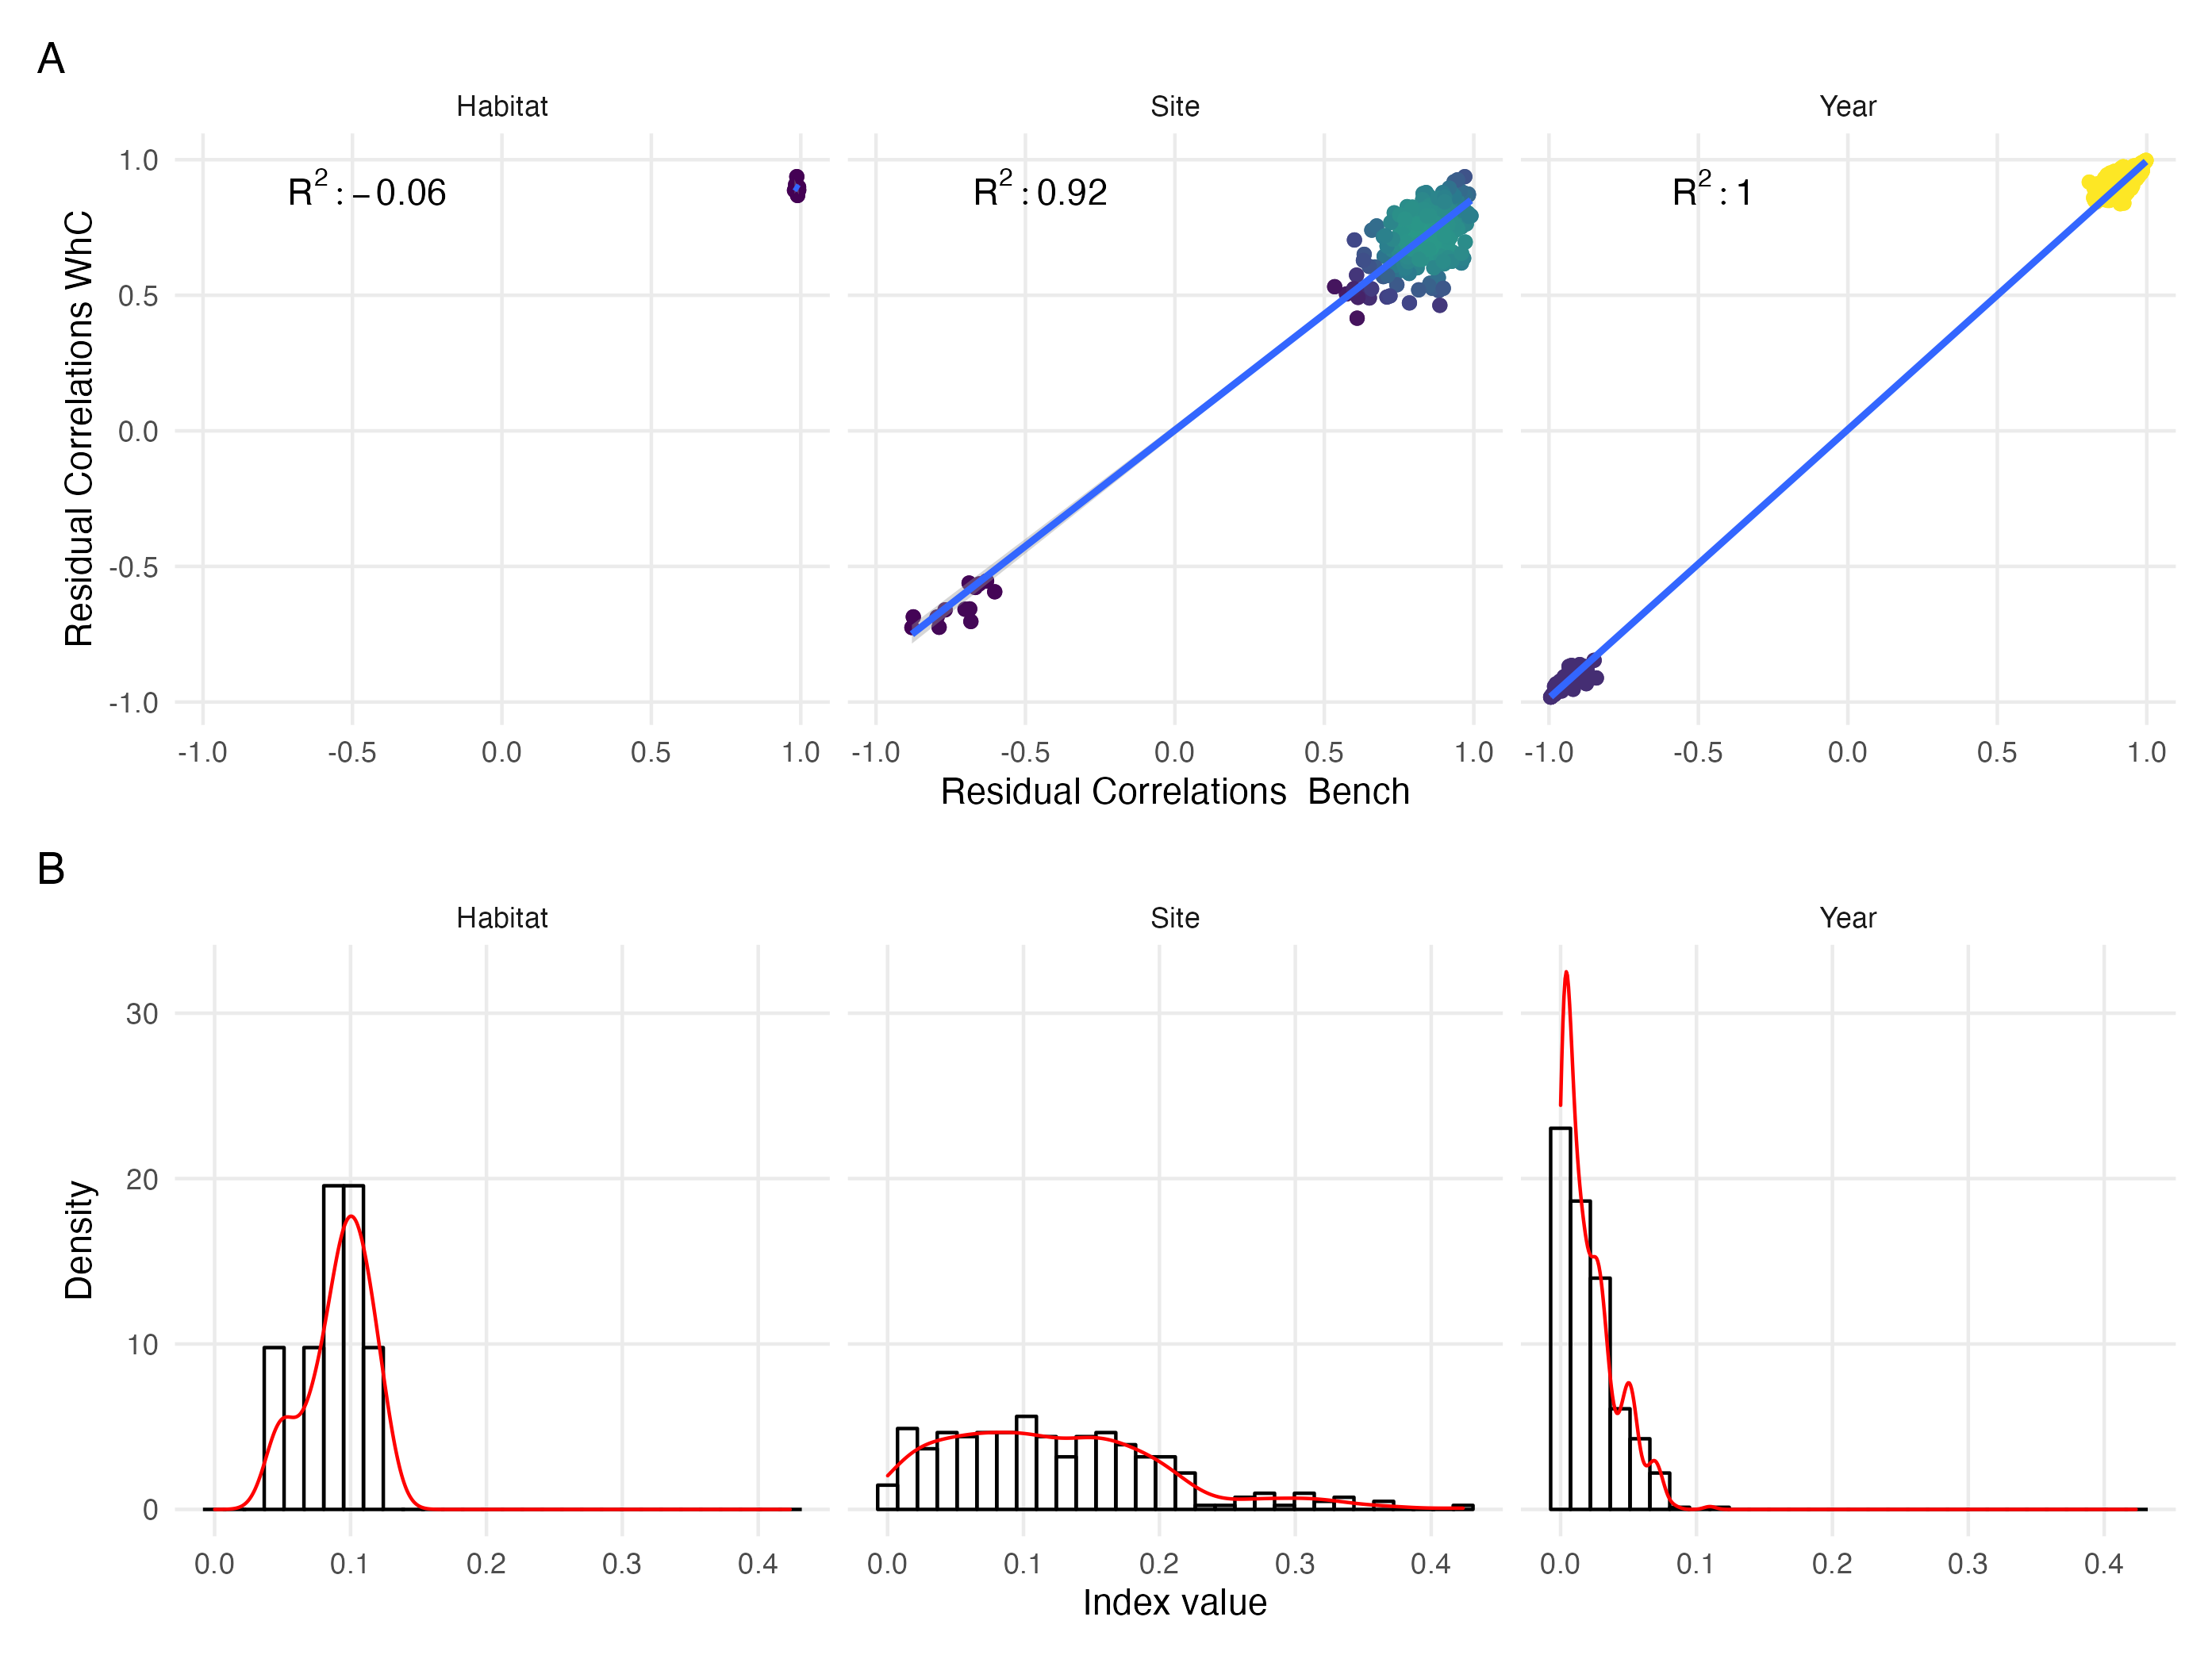
\includegraphics{figures/fig5.png}
\caption{Number (y-axis) and proportion (computed across all
coefficients for each model, as indicated above individual bars) of
response curves (i.e.~one for each species-predictor combination
according to the typology (nine shapes highlighted by the black curve in
each panel) defined by \textcite{Rigal_2020}. Results are presented for
the different model structures}\label{fig:chapt1fig5}
}
\end{figure}

Both abundance and presence/absence \emph{TrPh} models (which include
species functional traits) reveal some meaningful trait-environment
relationships between the first fuzzy-PCA axis and the seven
environmental predictors. This suggests that the occurrence of certain
traits is likely favored (or hindered) under certain environmental
conditions (Fig. S28). For instance, mobile predatory species showed
larger declines in abundance as fetch increases than sessile
suspensivores (Fig. S28). Moreover, increase in organic matter
concentration and decrease in current velocities were associated with
higher abundances of suspensive feeders.

\hypertarget{exploring-the-residual-correlation}{%
\subsection{Exploring the residual
correlation}\label{exploring-the-residual-correlation}}

Residual species-species correlations were compared between the
\emph{Bench} model and the \emph{WhC} model, only for the 99 target
species, using both presence/absence (Fig S29) and abundance data
(fig.~\ref{fig:chapt1fig6}). We only focus this comparison on the
\emph{WhC} model (rather than other models) because of its higher
predictive performance and higher proportion of explained variance by
random effects (fig.~\ref{fig:chapt1fig4}). Residual correlations
estimated from both models were highly correlated, both for
presence/absence and abundance data (fig.~\ref{fig:chapt1fig6} and Fig.
S29). However, agreement between models varied across different random
effects from a moderate correlation between residuals associated with
the Habitat random effects (\(\text{R}^2=0.57\)) or with the Site random
effects (\(\text{R}^2=0.64\)), to a high correlation between residuals
related to the Year random effects (\(\text{R}^2=0.95\)). The \(\delta\)
index main modal distribution, which is centered on zero, confirms an
overall agreement between residual correlations estimated from both
models in relation to the Year random effects with a marginal proportion
of sign changes (0.45\% of sign changes related to correlation greater
than 0.25; fig.~\ref{fig:chapt1fig6} B) only related to low
species-species residual correlations (\textless0.25;
fig.~\ref{fig:chapt1fig6} A and Fig. S29). In contrast, the \(\delta\)
index highlights inconsistencies in both magnitude and signs changes
between residuals associated with the Habitat and the Site (12.2\% and
9.11\% of sign changes related to correlation greater than 0.25) random
effects. Similar results were obtained for presence/absence models (Fig.
S29).

\begin{figure}
\hypertarget{fig:chapt1fig6}{%
\centering
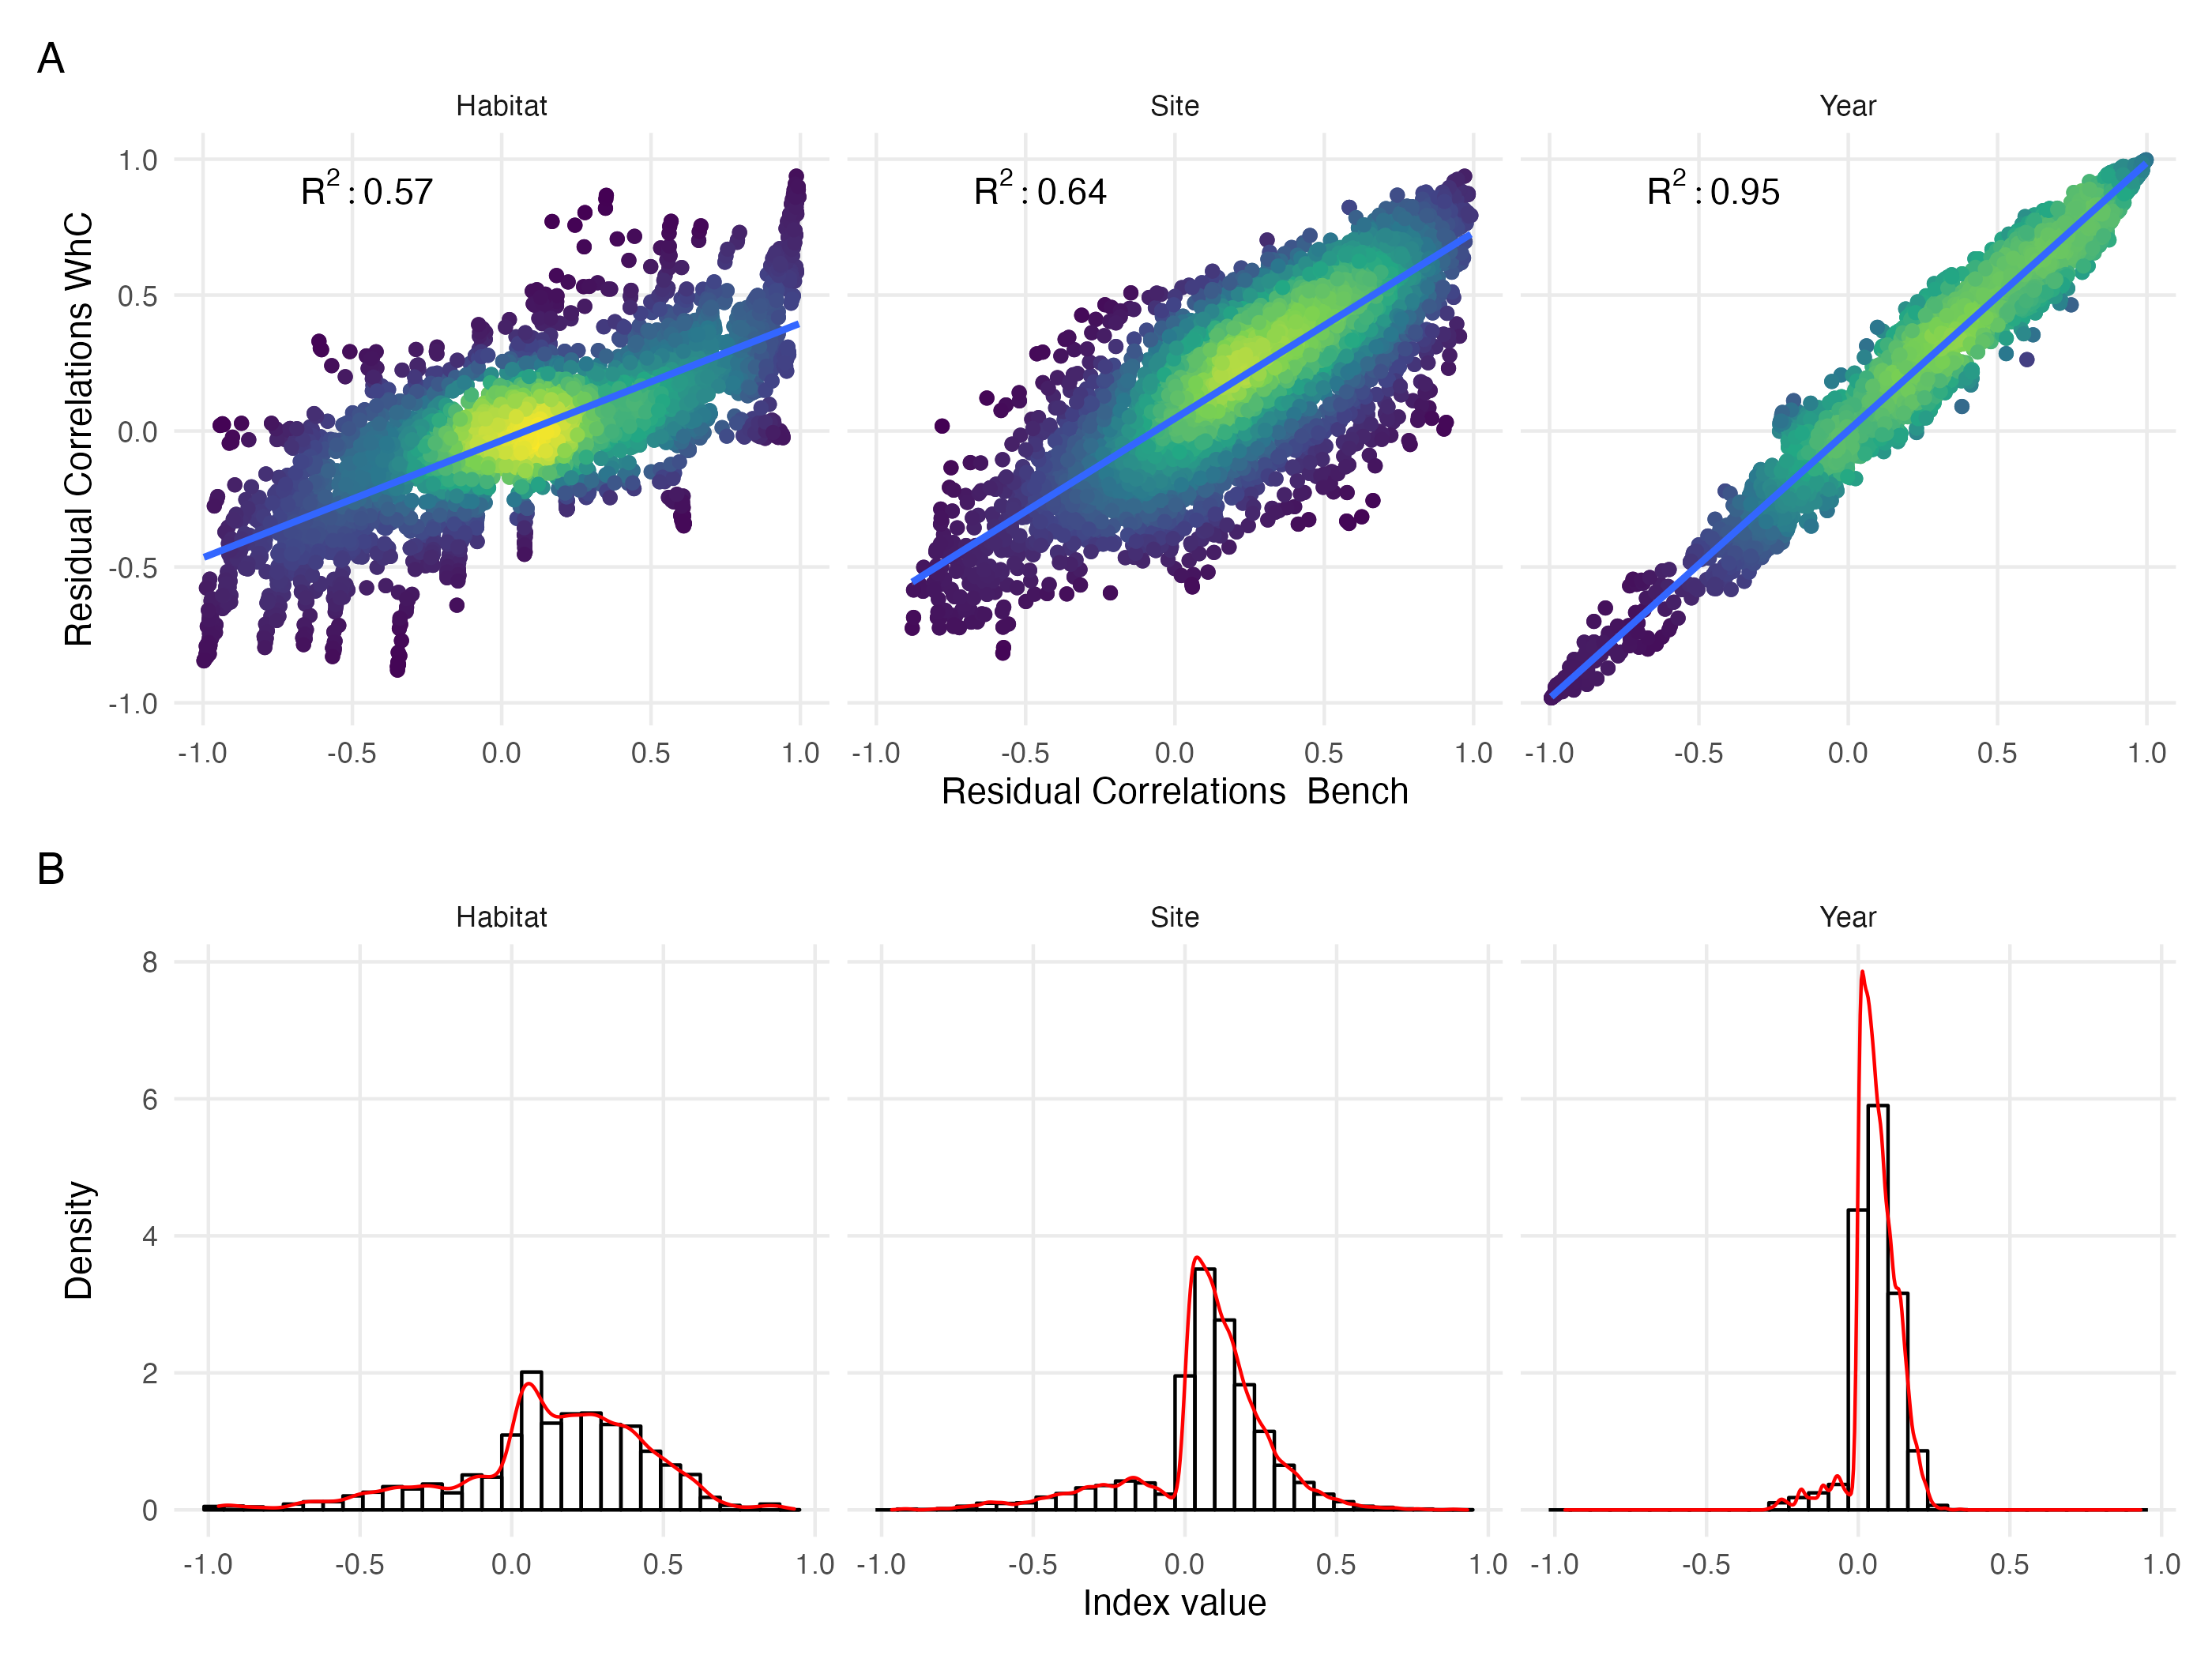
\includegraphics{figures/fig6.png}
\caption{(A) Comparison of residual species-species correlations
associated with the three random effects estimated by the \emph{Whole
Community Model} (\emph{WhC}; y-axis) and the \emph{Benchmark model}
(\emph{Bench}; x-axis) fitted on abundance data. The colour scale
highlights the density of points in each scatter plot. (B) Distribution
of the \(\delta\) index characterizing change in sign (negative values
indicate sign change) and magnitude (higher absolute values indicate
higher numerical difference) between residual correlations estimated by
the \emph{WhC} model and the \emph{Bench} model adjusted with abundance
data for the three random effects (Habitat, Site,
Year).}\label{fig:chapt1fig6}
}
\end{figure}

\hypertarget{discussion}{%
\section{Discussion}\label{discussion}}

Case studies in community ecology typically rely on partial and
heterogeneous observations \autocite{Pollock_2020} but also on
incomplete knowledge of target species ecological features (e.g.~traits,
phylogeny; \textcite{Tyler_2012}). This study investigated how
\emph{jSDM} performance varies depending on the type of information
included (i.e.~phylogeny, traits or data on non-target species) using a
multi-assessment framework (spanning interpretability, inference and
prediction, for both species- and community-level metrics, Table 1)
enabling a thorough evaluation of model performance.

We found that \emph{jSDMs}' performance, in particular predictive power
of abundance models at the species level, mostly increased when
including information related to the 179 non-target species sampled
alongside with the 99 polychaetes of interest. However, improvement in
species-level predictions does not directly translate into enhanced
performance at the community level. The \emph{WhC} model did not improve
estimates of beta diversity or total abundance relative to the other
models and largely overpredicted species richness, as previously
suggested \autocite{Zurell_2018}. Given \emph{HMSC} hierarchical
structure \autocite{Poggiato_2021}, inclusion of monitoring data related
to other species likely improves model performance for the target
assemblage by capturing relevant drivers that are not explicitly
considered. For instance, it can help describe target species' realized
niches by accounting for ecological processes related to environmental
conditions (including trait-mediated responses) or biotic interactions
that are not explicitly captured otherwise \autocite{Ovaskainen_2017a}.
In our case, main differences between residual correlations estimated by
the \emph{Benchmark model} and the \emph{Whole community} model relate
to spatial random effects (i.e.~site and habitat). In contrast, the
temporal random effect yielded similar residual co-occurrences in both
models. This suggests that including non-target species in our case,
mostly helped capture spatial variability in species associations across
sites and habitats.

Importantly, while we show that including non-target species can improve
predictive performance, in particular for rare species, benefits of
accounting for non-target species might vary depending on robustness of
non-target species monitoring data (e.g.~detection issues), their role
within the ecosystem (e.g.~engineer species are likely more influential
on local communities than rare transient species), or processes shaping
the target assemblage (if influence of abiotic factors dominates, then
adding other species will have marginal consequences on model
performance). While the list of additional species to consider can be
prioritized based on existing knowledge in well-studied ecosystems, such
information is often unavailable. Furthermore, a specific investigation,
that might rely on simulated datasets to overcome limitations related to
real world datasets \autocite{DiRenzo_2022}, would be required to
determine specific criteria, as well as optimal number of non-target
species to include. While species communities and assemblages are
largely defined arbitrarily \autocite{Stroud_2015}, a systematic
assessment of \emph{jSDM} performance as increasing the number and types
(for instance based on their functional or trophic roles) of non-target
species would be valuable to optimise model performance for the species
of management interests.

\emph{jSDMs} have already been used to model the distribution of a wide
variety of species ranging from micro-organisms \autocite{Minard_2019}
to megafauna \autocite{Brimacombe_2020} inhabiting many different
ecosystems. Here, while we studied assemblages associated with two
specific coastal habitats, i.e.~seagrass and sand, that have original
characteristics as they are located at the land-sea interface
\autocite{Boye_2019a}, our case study reflects typical aspects of
applied ecological research. These include issues related to data
limitation and availability but also typical features of ecological
communities (e.g.~prevalence of rare and transient species;
\textcite{Magurran_2003}) ; \textcite{SnellTaylor_2018}). Valuable
insights on trait-environment relationships are scarce in our study,
which reflects how contributions of functional ecology in \emph{jSDMs}
are likely limited by trait data quality and availability \autocites[
]{Tyler_2012}{deJuan_2022}. For instance, we found an interaction
between trophic modalities (i.e.~microphagous versus macrophagous diet)
and fetch (Fig. S15), indicating that organisms that filter on small
particles are less likely to occur in wave-exposed sites where high
levels of sediment resuspension can block their filtering systems
\autocite{Manning_2014}. Yet, the limited number of informative
trait-environment relationships or species-environment relationships
either suggest that neutral processes may shape polychaete assemblages
\autocite{Boye_2019a}; or rather highlight a mismatch between trait
data, environmental data, and the ecological processes at play
\autocite{deJuan_2022}. For instance, environmental variables only
capture mean climatological conditions, but fail to quantify variability
in the coastal environment, such as extreme events and seasonal or
annual variability. Likewise, the list of available fuzzy-coded traits
only partially captures species capacity to adapt to environmental
variability \autocite{deJuan_2022}. Thus, effectiveness of inclusion of
traits in \emph{jSDMs} is likely to be limited, or to rely on effort to
collect relevant trait information. In our case, while including traits
does not improve model predictive power, it somehow enhances our
understanding of species responses along environmental gradients. Hence,
if the goal is not prediction but inference \autocite{Tredennick_2021},
including traits and proxies of phylogeny can facilitate \emph{jSDM}
interpretation.

This paper lays out an original framework to systematically compare
multiple facets of alternative \emph{jSDM} formulations (i.e.~including
phylogeny, traits or additional species) on model interpretability,
explanatory and predictive power (Table 1). Using a set of complementary
metrics, we specifically assess performance of alternative model
formulations fitted to presence-absence or abundance data at the species
and community levels. Our framework goes beyond existing guidelines
proposed to assess the performance of \emph{jSDM} fitted on
presence-absence data \autocite{Wilkinson_2020} or that focus on the
predictive power of abundance-based models (e.g.
\textcite{Waldock_2022}). It specifically compares the performance (both
explanatory and predictive) and interpretability of alternative models'
formulations accounting for the multiple and high-dimensional components
that are typical of \emph{jSDMs}, namely: (1) species and community
level predictions including alpha and beta diversity metrics and ranking
of predictions according to species prevalence/abundance; (2)
species-environment relationships where we transposed the framework
initially developed for time series by \textcite{Rigal_2020} into an
effective tool to classify response curves according to 9 categories
across high numbers of species (e.g.~99 in our case study); (3)
trait-environment relationships; and (4) residual species-species
correlations associated with random effects thanks to a new index that
summarizes both changes in the sign and magnitude of the residual
correlations.

Overall, our results provide new insights into the most appropriate
strategies for \emph{jSDM} fitting, according to modelling objectives
\autocite{Tredennick_2021} and available data. While the four models
considered had similar explanatory power, adding extra information to
standard \emph{jSDMs} that only consider abiotic predictors can prove
useful in cases. For instance, adding monitoring data for other
non-target species can substantially increase model predictive power by
modifying inferred species-environment relationships and residual
correlation matrices. Similarly, adding traits or phylogeny can improve
model interpretability. Future studies will be key to consolidate our
findings on simulated case studies \autocites[
]{Zurell_2010}{DiRenzo_2022}, or across contrasted ecosystems, for
instance dominated either by environmental filtering, or by competitive
processes. Generalizing this approach across ecosystems will further
help prioritize data collection effort on the long term. For this
purpose, we recommend using a multi-model inference framework similar to
the one used in this study to systematically assess trade-offs
associated with alternative jSDMs formulations.

\hypertarget{author-contributions}{%
\subsection{Author Contributions}\label{author-contributions}}

MPM conceived the project with inputs from CV, AB, MC. CV analysed data
and led manuscript write-up. All authors had significant inputs to the
manuscript and approved this final version.

\hypertarget{acknowledgments}{%
\subsection{Acknowledgments}\label{acknowledgments}}

We are grateful to Marion Maguer and Vincent Le Garrec who conducted
fieldwork and laboratory analyses, as well as to supporting students and
staff involved in the REBENT monitoring programme coordinated by
Sandrine Derrien (MNHN) and its funding partners (Agence de l'eau
Loire-Bretagne, Région Bretagne, DREAL Bretagne). The authors would also
like to acknowledge the Pôle de Calcul et de Données Marines (PCDM) for
providing DATARMOR storage and computational resources.
\url{https://pcdm.ifremer.fr}. MPM is the recipient of an ANR early
career grant ANR-21-CE02-0006.

% DON'T EDIT. If "endfloat" option is enabled all floats appear before appendices
\if@endfloat\clearpage\processdelayedfloats\clearpage\fi 

\printbibliography[heading=bibintoc, title={References}]

%%%%%%%%%%%%%%%%%%%%%%%%%%%%%%%%%%%%%%%%%%%%%%%%%%%%%%%%%%%%
%%% SUPPLEMENTARY MATERIAL / APPENDICES
%%%%%%%%%%%%%%%%%%%%%%%%%%%%%%%%%%%%%%%%%%%%%%%%%%%%%%%%%%%%
%% Sadly, we can't use floats in the appendix boxes. So they don't "float", but use \captionof{figure}{...} and \captionof{table}{...} to get them properly caption.


% % appendixbox not supported

% \begin{appendix}
% \end{appendix}

%%%%%%%%%%%%%%%%%%%%%%%%%%%%%%%%%%%%%%%%%%%%%%%%%%%%%%%%%%%%
%%% ARTICLE END
%%%%%%%%%%%%%%%%%%%%%%%%%%%%%%%%%%%%%%%%%%%%%%%%%%%%%%%%%%%%

\end{document}
